\documentclass{article}
\usepackage[a4paper, right=2cm, left=2cm, top=2cm,
bottom=2cm, bindingoffset=0.5cm]{geometry} % margins
\usepackage{parskip} % no paragraph
\usepackage{hyperref} % link referencing
\usepackage{booktabs} % enhancing tables
\usepackage{multicol} % multicolumns
\usepackage{graphicx} % adding external figures
\usepackage{enumitem} % itemization
% equations
\usepackage{amsmath}
\usepackage{amsthm}
\usepackage{amssymb}
\usepackage{mathtools} % extra arrows
\usepackage{textcomp} % using only for degrees
\usepackage{siunitx} % scientific notations
\usepackage{cancel} % extra notations
% equations
\usepackage[version=4]{mhchem} % chemical formulas
\usepackage{fancyhdr} % custom headers and footers
\usepackage{caption} % for custom captions
\usepackage[
backend=biber,
sorting=anyvt,
style = ieee
]{biblatex} % for using references
\addbibresource{course.bib}

% tikz packages
\usepackage{tikz}
\usetikzlibrary{positioning}
% tikz packages

% page style
\pagestyle{fancy}
\fancyhead[L]{\textbf{Middle East Technical University}}
\fancyhead[R]{\textbf{ENVE422}}
\fancyfoot[L]{Treatment and Disposal of Water \& Wastewater Sludge}
\fancyfoot[C]{}
\fancyfoot[R]{Page \thepage\ of \pageref*{LastPage}}
\renewcommand{\headrulewidth}{0.4pt}
\renewcommand{\footrulewidth}{2pt}
\setlength{\headheight}{15pt}
\addtolength{\topmargin}{-3pt}
% page style

% items
\setlist[itemize]{leftmargin=*}
\setlist[enumerate]{leftmargin=*}
\renewcommand{\labelenumii}{\arabic{enumi}.\arabic{enumii}}
\renewcommand{\labelenumiii}{\arabic{enumi}.\arabic{enumii}.\arabic{enumiii}}
\renewcommand{\labelenumiv}{\arabic{enumi}.\arabic{enumii}.\arabic{enumiii}.\arabic{enumiv}}
% items

% captions
\DeclareCaptionListFormat{figure}{Figure #1#2.}
\DeclareCaptionListFormat{table}{Table #1#2.}
\captionsetup[figure] {font=it, labelsep=period, labelfont=bf, listformat = figure}
\captionsetup[table] {font=it, labelsep=period, labelfont=bf, skip = 5pt, listformat = table}
\renewcommand{\numberline}[1]{#1\ } 
\counterwithin{figure}{section}
\counterwithin{table}{section}
\numberwithin{equation}{section}
% captions

% linespacing
\linespread{1.25}
% linespacing

\title{{\Large EnvE422 - Lecture Notes}\\ {\large Treatment and Disposal of Water \& Wastewater Sludge}\\{\normalsize Middle East Technical University}}
\author{\href{mailto:sahin.bekir@metu.edu.tr}{\small Bekir Şahin}}
\date{\small Spring 2023} % not sure about the title

\begin{document}
\maketitle
\tableofcontents
\setcounter{page}{0}
\thispagestyle{empty}
\newpage
\listoftables
\listoffigures
\date{\begin{flushright}March 10, 2023\end{flushright}}
\section*{Syllabus}
\textbf{Comment from the instructor:} It is a hard course!
\subsection*{Introduction}
General premise: Provides general information on how general sludge is handled.\\
\textit{Cradle to cradle} approach to sludge: How much sludge production, the characteristics of the sludge, how it can be made use of it beneficially...
\subsection*{Grading}
\begin{itemize}[align=left, itemindent=*]
    \item[!] \textbf{No midterm for the course.} 
    \item[\textbf{30\%}] Quiz, almost every other week. One bad quiz will be excluded. 
    \item[\textbf{25\%}] Team presentation, also have to contribute to the discussion! Presentation, 2 page summary, 1 question in the final exam from each.
    \item[\textbf{35\%}] Final.
    \item[\textbf{10\%}] 3, 4 homework!
    \item[\textbf{5\%}] Participation (extra).
\end{itemize}
\subsection*{References}
\fullcite{sanin_clarkson_vesilind_2011} $\Rightarrow$ \textbf{Nice reference, complimentary to the course (extra reading and concepts), further example questions can be found.}\\
\fullcite{vesilind_hartman_skene_1988} $\Rightarrow$ \textbf{Quite old, design-based, a case study included for a holistic approach.}\\
\fullcite{tchobanoglous_stensel_tsuchihashi_burton_2014} $\Rightarrow$ \textbf{General concepts for wastewater engineering, design-based.}
\newpage
\date{\begin{flushright}March 17, 2023\end{flushright}}
\section{What is Sludge?}
How to use Sludge?
\begin{enumerate}
    \item Fertilizer
    Stabilization by reducing the microbial activity.
    \item Incineration $\Rightarrow$ it has some calorific value, drying is a must.\\
    Brown coal, lignite (which is found in Turkey). Almost same in terms of calorific value.
\end{enumerate}
Three important rules while handling sludge:
\begin{enumerate}
    \item Don't hold sludges!
    \item Don't mix sludges!
    \item Don't recirculate sludges!
\end{enumerate}
\subsection{Sludge Quantification}
Semi-solid material produced by water and wastewater treatment that itself needs further treatment for disposal into the environment. The amount depends on the \emph{quality of wastewater} incoming.
Why treatment?
\begin{itemize}
    \item High organic content
    \item Nutrients
    \item Pathogenic microorganisms
    \item Lots of water
\end{itemize}
Typical sludge generation (by census data and sludge production data): 0.025--0.095 kg/capita/day\\
\textbf{In Turkey:} 0.035 kg/capita/day\\
Numbers depends on:
\begin{itemize}
    \item Wastewater characteristics
    \item Treatment types in the system
    \item Sludge treatment units
\end{itemize}
Although, the temperature, the climate, etc. are parameters, those three are the most affecting ones.\\
Sources:
\begin{itemize}
    \item Wastewater treatment:
    \begin{enumerate}
        \item Primary\\
        Primary treatment $\rightarrow$ For settleable solids with some intention of BOD\\
        Screens, disposed in landfills, no more treatment\\
        Primary treatment, called raw primary sludge, which has very objectionable properties:
        \begin{itemize}
            \item Odor
            \item Organics
            \item Water content
            \end{itemize}
            Therefore, it should be treated.\\
            Typical treatment: anaerobic digesters, dewatering.\\
            Digesters do further treatment, then dewatering (reduces water content) process comes along.\\
            Then, it can be used for beneficially.\\
            Anaerobic digesters do:\begin{itemize}
                \item Organic content reduction
                \item Objectionable odor removal
                \item Pathogens reduction
            \end{itemize}
        \item Secondary\\
        Secondary treatment $\rightarrow$ For removing BOD\\
        In advanced systems we don't have primary clarifier, final clarifier, returned activated sludge.\begin{enumerate}
            \item Return activated sludge: coming from final clarifier back to aeration chamber.
            \item Waste activated sludge: rest of the microbial flocs is removed from the system.
            \item Waste activated sludge + Raw primary sludge: to digester (almost 50/50 to be stabilized)
        \end{enumerate}
    \item Water treatment (Totally different)\\
    Water treatment $\rightarrow$ settling tank (major source)\\
    Does not go to digester, first to thickener, then dewatering.\\
    Water treatment sludge (different from wastewater), the amount affected by added coagulant, the quality of the water, and the scheme of the water treatment plant.\\
    Digestion  refers to the organic removing (for biomass), so no need for a chemical sludge.\\
    Thickening refers to squeezing the water.\\
    It is handled as an industrial sludge (landfilling).
    \item Industrial Sludge $\rightarrow$ hazardous waste (not included in this course)
    \end{enumerate}
\end{itemize}

\begin{table}[htbp]
    \caption{\label{tab:sludge_types}Types of sludge, their physical concentrations and characteristics.}
    \centering
    \begin{tabular}{p{0.3\linewidth}rp{0.4\linewidth}}
        \toprule
        Sludge & Conc. (\%) & Characteristics \\
        \midrule
        Raw primary & 4--8 & not drained well on drying beds \newline dewatered mechanically\\
        Anaerobic primary digested & 6--10 & gas production, well on drying beds\\
        Wasted activated sludge & 0.5--1.5 & no odor, but bio. active\\
        Mixed digested & 2--4 & produces gas, not as easy to dewater\\
        Aerobic digested & 1--3 & bio. active, not as easy to dewater\\
        Waste alum & 0.5--1.5 & not active, inorganic content\\
        \bottomrule
    \end{tabular}
\end{table}

Nitrogen, ammonia, nitrate, phosphorus, potassium are important for fertilizer and exists in sludge.\\
Sodium, calcium iron are some inorganic content in the sludge.\\
Microorganisms: Viruses, fecal coliforms, \textsl{Salmonella} \ldots\\
Before and after $\rightarrow$ they are still there after the treatment.

\begin{figure}[htbp]
    \centering
    
\includegraphics[width=0.95\textwidth]{SludgeQuantities.png}
    \caption{Flow chart of a sludge generation in a conventional wastewater treatment plant.}
    \label{fig:sludge}
\end{figure}
\begin{center}\textbf{\Large Mass Balance Approach}\end{center}
\textbf{\large Parameters}\\
S$_0$ = influent BOD (kg/h)\\
X$_0$ = influent suspended solids (kg/h)\\
Those are \textbf{loads}.\\
k = fraction of X$_0$ removed in the primary clarifier\\
From primary, kX$_0$ to digester $\Rightarrow$ \textbf{up to 0.6} for k, good number if close to this.\\
h = fraction of BOD \textbf{not removed} in the primary clarifier\\
hS$_0$ and (1-k)X$_0$ $\Rightarrow$ h is \textbf{0.7 minimum}, means \textbf{30\% removed} with primary clarifier, since we are not removing BOD in the primary clarifier, it is expected.\\
i = fraction of BOD \textbf{not removed} in the aeration tank\\
X$_f$ = plant effluent suspended solids (kg/h)\\
\textbf{After final clarifier:}\\
ihS$_0$ $\Rightarrow$ so i has to be \textbf{really small} (0.1, means \textbf{90\% removal}) and X$_f$ after the removal.\\
j = fraction of solids \textbf{not destroyed} in digester\\
$\Delta$X = net solids produced by biological action (kg/h)\\
Y = Yield = $\Delta$X/$\Delta$S, where:\\
$\Delta$S = hS$_0$ - ihS$_0$\\
\textbf{Incoming to digesters and after treatment:}\\
1$^{\text{st}}$: kX$_0$ came, as primary only jkX$_0$, j = 0.8 means \textbf{20\% removal} achieved for primary only.\\
2$^{\text{nd}}$: (1-k)X$_0$-X$_f$ + $\Delta$X\\
$\Delta$X is net solids produced by biological action.\\
Y (Yield) = $\Delta$X/$\Delta$S\\
\textbf{\large Typical Values}
\begin{itemize}
    \item S$_0$ = 250 * 10$^{-3}$ * Q = kg/h,\\
    here 250 mg/L and Q = m$^3$/h
    \item X$_0$ = 225 * 10$^{-3}$ * Q = kg/h,\\
    here 225 mg/L and Q = m$^3$/h
    \item h = 0.7
    \item i = 0.1 for well-operated activated sludge
    \item i = 0.2 for trickling filters (less treatment)
    \item X$_f$ = 20 * 10$^{-3}$ * Q = kg/h,\\
    here 20 mg/L and Q = m$^3$/h
    \item k = 0.6
    \item j = 0.8 (assuming no supernatant withdrawal)
    \item Y = 0.5 for activated sludge
    \item Y = 0.2 for trickling filters, because it is bio-film.
\end{itemize}
\subsection{Sludge Characteristics}
Differences are caused due to differences in \emph{the type and quality of wastewater} and \emph{differences in the wastewater treatment processes and operations}.\\
General sludge characteristics by typical parameters can be explained (even though it is time dependent).\\
\textbf{Physical characteristics:}
\begin{enumerate}
    \item Specific gravity\\
    \textbf{Definition:} Ratio of  weight of the material to the weight of an equal volume of water.\\
    1L sludge weighing 1010 g / 1000 g water = 1.01 is the specific gravity.\\
    Most sludge have specific gravity of 1.0, almost equal to the weight of water, what might be the problem?\\
    \emph{Shows similar behavior as water with gravity, physical separation is hard.}\\
    Sludge is suspension, solid and liquid and more than one solid (volatile and fixed components exist):
    \[
    \frac{1}{S} = \sum_{i=1}^{n} \frac{W_i}{S_i}
    \]
    where:\\
    $S$ = specific gravity of the sludge,\\
    $W_i$ = weight fraction of the $i^\text{th}$ components of sludge,\\
    $S_i$ = specific gravity of the $i^\text{th}$ component.
    \item Sludge density\\
    Again, very close to 1 (1.0\_ in examples).
    \item Solid concentration\\
    mg/L or \% (w/w) solids\\
    From X\%:
    \[
    \frac{X\text{ kg}}{100\text{ kg}} * \rho_\text{sludge}\text{ (kg/m}^3\text{)} * \frac{10^6\text{ mg}}{\text{kg}} * \frac{\text{m}^3}{10^3\text{ L}} = \text{mg/L}
    \]
    if we assume the specific gravity of the slurry is 1.0 (it is slightly higher than that in reality),\\
    10,000 mg/L = 1\%\\
    For sludge with higher S values, the relationship will change.\\
    \textbf{Solid content and types:}
    \[
    \text{Total Solids} = \text{Suspended Solids} + \text{Dissolved Solids}
    \]
    \[
    \text{Total Solids} = \text{Volatile Solids} + \text{Fixed Solids}
    \]
    \[
    \text{\% Solids} = 100 - \text{\% Moisture}
    \]
    \item Settling characteristics\\
    How well it settles.
    \begin{itemize}
        \item Zone Settling Velocity (Hindered settling test) (ZSV)\\
        ZSV is in hyperbolically inverse relationship with concentration.
        \[
        \text{Zone Settling Velocity (ZSV)} \propto \frac{1}{C}
        \]
        Why is there such a relationship?\\
        \emph{Higher concentration compresses in more time, the already settled particles creates interference.}\\
        Why do we care settling in second?
        \begin{itemize}
            \item If not good settling, the return sludge will be low.\\
            return sludge is essential $\rightarrow$ maintaining a good solid content, good MLSS results in good removal.
            \item If not settle, we lose them to effluent, all the work we did is gonna be wasted.
        \end{itemize}
        \item Sludge Volume Index (SVI)\\
        Quick test.\\
        1L cylinder for 30 min.
        \[
        \text{SVI} = \frac{V_{30}*1000}{\text{MLSS}}
        \]
        where:\\
        SVI = Sludge Volume Index (volume occupied by 1 gram of solids, mL/g, but unitless),\\
        $V_{30}$ = sludge volume settled in 30 minutes, volume unit,\\
        1000 = conversion factor (1000 mg/g),\\
        MLSS = Mixed Liquor Suspended Solids, concentration unit.\\
        An operational tool designed for the  treatment, more about settleability to gain an idea but not a good research too. Because it is not independent of solid concentration, may result in bad cases for both extremely low and high concentrations. Greater than 7000--8000 mg/L is misguiding, not settled (1000 mL sludge with) 10000 mg/L MLSS content gives 100 as SVI value, which is good in terms of numbers but in reality it is bad. The \textbf{concentration}, \textbf{diameter} of the cylinder, \textbf{length} of the cylinder affects the outcome of the test.
\begin{itemize}
    \item $40 < \text{SVI} < 120$ $\Rightarrow$ well-settling
    \item $\text{SVI} > 120$ $\Rightarrow$ bulking sludge
    \item $\text{SVI} > 150$ $\Rightarrow$ severely bulking sludge, requires action.
\end{itemize}
        \item Particle size\\
        Micro-level, cannot be defined by a single size $\Rightarrow$ a distribution must be mentioned.
        Many dynamic affect the distribution. The uniformity can be examined by using a power law model:
        \[
        \frac{d\text{N}}{d\text{L}} = \text{AL}^\beta
        \]
        where:\\
        N = density of particles,\\
        L = length of particles.\\
        log(L) vs. log($\Delta$N/$\Delta$L) graph yields $\beta$ coefficient. The $\beta$ coefficient is closer to 1, it is more uniform in terms of distribution. Viscosity, settling, dewatering are affected.\\
        Measurement is hard.
        \begin{itemize}
            \item Filtration, thorough a series of different sized filters.
            \item Photographic techniques.
            \item Scattering laser light.\\
            Even you measure, dewatering settling rheology is still complicated.
        \end{itemize}
        \item Floc structure and porosity\\
        Flocs formed from three major components:
        \begin{itemize}
            \item microorganisms
            \item extracellular polymers
            \item water
        \end{itemize}
        Extracellular polymers (EPS) hold individual microorganisms $\Rightarrow$ flocs causes separation.\\
        Filamentous organisms give strength to the structure.\\
        EPS is a major component, creates a structure with water channels, gaps, reservoirs.\\
        It has pores: \textbf{porosity}.\\
        Activated sludge porosity: 0.999; 0.91 $\pm$ 0.15 (in another study).
        \end{itemize}
    \end{enumerate}
\date{\begin{flushright}March 24, 2023\end{flushright}}
\begin{enumerate} [start=5]
    \item Distribution of Water in Sludge\\
    Sludge is two-phase slurry.\\
    To carry the sludge, we must minimize the volume of the sludge. Form of water in sludge determines the effectiveness of sludge treatment.\\
    Besides drying, freezing is a good option for dewatering. Freezing does not happen at 0\textdegree C or lower like -3\textdegree C, it happens -20\textdegree C.\\
    Constituents of sludge:\\
    \textbf{Free (bulk) water (75\%):} Water not associated with solids and not influenced by solids.\\
    \textbf{Interstitial water (20\%):} Water trapped in the interstitial spaces of the flocs and organisms. This part can be removed by mechanical dewatering.\\
    \textbf{Vicinal water:} Multiple layers of water molecules help tightly to the particle surface by hydrogen bonding. Very hard to remove, it exists as long as there is a surface. The binding force is really strong.\\
    \textbf{Lower density}, \textbf{higher viscosity} compared to bulk water. Very critical part!\\
    \textbf{Water of Hydration:} Chemical bound water with the particles, only removable with the expenditure of thermal energy (ex. drying).\\
    dewatering $\Rightarrow$ 20\% water removal\\
    thermal drying $\Rightarrow$ 95\% water removal
    \item Rheology\\
    Science of flow and deformation of fluids.\\
    Commonly measured in terms of \textbf{viscosity}.\\
    Shear force applied, a velocity distribution occurs.
    \begin{enumerate}
    \item Newtonian fluids:
    \[
    \tau = \mu \frac{du}{dy}
    \]
    where:\\
    $\tau$ = shear stress (N/m$^2$ or Pa),\\
    $\mu$ = viscosity (Pa·s),\\
    $du/dy$ = shear rate (1/s).\\
    Viscosity is dependent on temperature.\\
    Sludge $\Rightarrow$ mostly not Newtonian but if it is diluted it is Newtonian.
    It is not about thickness, thick fluids can be Newtonian.
    \item Bingham plastic fluids:
    \[
    \tau = \tau_y + \eta \frac{du}{dy}
    \]
    where:\\
    $\tau$ = shear stress (N/m$^2$ or Pa),\\
    $\tau_y$ = yield stress (N/m$^2$ or Pa),\\
    $\eta$ = plastic viscosity (Pa·s),\\
    $du/dy$ = shear rate (1/s).\\
    There is a intercept (yield stress, that should be overcome to make the fluid flow) in the formula, but it looks like Newtonian.
    \item Pseudoplastic fluids:
    \begin{equation}
        \tau = K \left(\frac{du}{dy}\right)^n
        \label{eq:powerlawmodel}
    \end{equation}
    where:\\
    $\tau$ = shear stress (N/m$^2$ or Pa),\\
    \textbf{Most} wastewater sludges are neither Newtonian nor plastic non-Newtonian.\\
    K = fluid consistency index, analogous to viscosity,\\
    n is flow behavior index,\\
    n $<$ 1 for this sludge flow.
    \item Dilatant fluids:\\
    We don't see that in sludge. Same as pseudoplastic fluid (power law model), but n $>$ 1.\\
    Sludge is believed to be a mix of pseudo-plastic and plastic, which means with a intercept decreasing curve.
    \end{enumerate}
Viscosity of sludge changes over time. It is a \textbf{thixotropic fluid}, since we break flocks while adding shear stress, a hysteresis (it does not follow the same curve) loop occurs.\\
\textbf{Einstein's Equation of Viscosity:}
\[
\mu = \mu_0 (1+2.5\phi)
\]
where:\\
$\mu_0$ = viscosity of suspending medium,\\
$\phi$ is the volume fraction of particles.\\
The particles in the medium increases the viscosity, follows 10\% volume fraction but this is for molecules that don't interact with each other.\\
4 parameters: \emph{shear stress}, \emph{time of measurement}, \emph{temperature}, \emph{solids concentration}.
\item Dewaterability
\begin{enumerate}
    \item Specific Resistance to Filtration as a Dewaterability Indicator:\\
    Belt filter, vacuum filter were mostly based on filtration.\\
    Now, it is based on centrifugation.
    Darcy's law is based.
    \[
    \frac{dV}{d\theta} = \frac{PAK}{\mu L}
    \]
    where:\\
    $dV/d\theta$ = rate of flow, volume per unit time,\\
    $P$ = pressure difference,\\
    $A$ = area,\\
    $\mu$ = viscosity,\\
    $K$ = permeability,\\
    $L$ = thickness.\\
    Carman -- Kozeny adapted Darcy's law for filtration. The resistance is contributed by the filter medium and the cake. Coakley and Jones adapted Carman's theory.\\
    For an expression with \textsl{Resistance}  (Resistance for sludge is better term so $R = 1/K$):
    \[
    \frac{dV}{d\theta} = \frac{PA}{\mu LR}
    \]
    where:\\
    $R$ = resistance ($1/K$).\\
    \textbf{Considering filter resistance with the cake resistance:}
    \begin{equation}
        \frac{dV}{d\theta} = \frac{PA}{\mu (LR+R_f)}
    \label{eq:dar1}
    \end{equation}
    where:\\
    $R_f$ = resistance of filter medium.\\
    The volume of filter cake can be expressed as:
    \[
    LA = vV
    \]
    where:\\
    $v$ = volume of cake deposited per unit volume of filtrate ($V$),\\
    Substituting L in Equation \ref{eq:dar1}:
    \[
    \frac{dV}{d\theta} = \frac{PA^2}{\mu (RvV+R_fA)}
    \]
    It is more convenient to express the cake as dry weight of cake deposited per unit volume of filtrate ($w$). $R$ (resistance by a unit volume) is also changed with $r$ (resistance per unit weight).
    \[
    \frac{dV}{d\theta} = \frac{PA^2}{\mu (rwV+R_fA)}
    \]
    where:\\
    $w$ = weight of dry cake solids per unit volume of filtrate,\\
    $r$ = specific resistance per unit weight.\\
    Assuming constant pressure over time:
    \begin{equation}
        \smallint_{0}^{\theta} d\theta = \smallint_{0}^{V} \left( \frac{\mu rwV}{PA^2}+\frac{\mu R_f}{PA}\right)dV \label{eq:dar2}
    \end{equation}
    Integrating Equation \ref{eq:dar2}:
    \begin{equation}
        \frac{\theta}{V} = \frac{\mu rwV}{2 P A^2} + \frac{\mu R_f}{P A} \label{eq:dar3}
    \end{equation}
    Using Equation \ref{eq:dar3}, experimental data can be obtained by plotting $\theta/V$ and $V$ values on a graph to yield a linear relationship.
    \[
    y=mx+b
    \]
    where:\\
    $y = \theta/V$\\
    $m = \text{ slope } = \mu rw / 2 PA^2$\\
    $x = V$\\
    $b = \text{ intercept } = \mu R_f / PA$\\
    $r$ can be obtained by using slope:
    \[
    r = \frac{2 P A^2 m}{\mu w}
    \]
    They were noisy, electricity use too much, too much space.\\
    Specific resistance = Buchner funnel apparatus.\\
    Definitely gives you dewaterability with filtration based system
    inorganic/non-inorganic compressible minerals, vacuum filtration is used.\\
    Check Equation \ref{eq:liqbalance} and Equation \ref{eq:solidsbalance} for the following expression:
    \begin{equation}
        w = \frac{Q_KC_K}{Q_F} \label{eq:w_1}
    \end{equation}
    Substituting Equation \ref{eq:liqbalance}:
    \[
    w = \frac{(Q_0-Q_F)C_K}{Q_F}
    \]
    Rearranging Equation \ref{eq:solidsbalance} with Equation \ref{eq:liqbalance}:\\
    \(Q_FC_F=Q_0C_0 - Q_KC_K\)\\
    \(Q_FC_F=Q_0C_0 - (Q_0-Q_F)C_K\)\\
    \(Q_FC_F=Q_0C_0 - Q_0C_K+Q_FC_K\)\\
    \(Q_FC_F -Q_FC_K = Q_0C_0 - Q_0C_K\)\\
    Rearranging the formula:
    \begin{equation}
        Q_F = \frac{Q_0(C_0-C_K)}{C_F-C_K} \label{eq:w_2}
    \end{equation}
    For $w$, if the filtrate SS can be assumed negligible (which is reasonable), i.e., $C_F$ = 0, and as Equation \ref{eq:w_2} is substituted into Equation \ref{eq:w_1}, then:
    \[
    w = \frac{C_KC_0}{(C_K-C_0)}
    \]
    If in \%:
    \[
    w = \frac{C_KC_0}{100(C_K-C_0)}
    \]
    where:\\
    $C_K$ = cake solids concentration (\%),\\
    $C_0$ = feed solids concentration (\%).\\
    A new test is developed, which is CST (capillary suction time).
    \item CST (capillary suction time):\\
    Gives an idea for 1 cm movement of water, developed in England national lab, comparing sludge, best conditioners function of:
    \begin{enumerate}
        \item CST filter properties (depth, thickness, etc.)
        \item Instrument properties (diameter of the open part)
        \item Sludge related properties (solid concentration, filtrate viscosity, sludge cake permeability)
    \end{enumerate}
    It is an empirical model by Vesilind:
    \[
    \chi = (D_2^2 - D_1^2)\left(\frac{\pi d}{ A P }\right)\left(\frac{\mu C}{t}\right)
    \]
    where:\\
    $D_1$ = 1$^\text{st}$ sensor location (diameter, m),\\
    $D_2$ = 2$^\text{nd}$ sensor location (diameter, m),\\
    $d$ = filter paper depth (thickness, m),\\
    $A$ = area of the bottom of the collar (sludge area, m$^2$),\\
    $P$ = capillary suction, analogous to head term in Darcy's equation (m),\\
    $\mu$ = filtrate viscosity (N·s/m$^2$),\\
    $C$ = sludge solids concentration (kg/m$^3$),\\
    $t$ = capillary suction time (s),\\
    $\chi$ = sludge filterability incorporating permeability (kg$^2$/m$^4$·s$^2$).
    \begin{itemize}
        \item Instrumental: sensors, paper thickness, collar size, paper absorbency.
        \item Sludge related: sludge sample, fluid viscosity, solids concentration.
    \end{itemize}
    SRF $\Rightarrow$ higher, harder to filter, related to resistance.\\
    $\chi$ $\Rightarrow$ higher (because it is in inverse relation with CST value), easier to filter, related to filterability.\\
    They are both independent, both are good, SRF is easier to measure but correlations help.
\end{enumerate}
\end{enumerate}
\textbf{Chemical characteristics:}\\
Presence of organic materials make it complicated.\\
Important for the final destination of sludge.
\begin{enumerate}
    \item Calorific value\\
    Dry sludge has a fuel value up to 5500 cal/g dry volatile solids (not a bad number), Coal has a fuel value of 7700 cal/g, very good coal.\\
    Unfortunately, sludge neither dry not it contains only the organics, which gives 550 cal/g.\\
    Combustion of sludge usually requires the use of auxiliary fuel, treatment decreases the calorific value.\\
    66\% Turkish lignite around 1000 and 2000.\\
    For industrial sludges, the calorific values varies. Most of them are higher than the lignite in Turkey.\\
    Municipal sludge average is \textbf{3580 kcal/kg}. And they don't show much variations. \textbf{Stabilization} processes change the calorific value.
    \item Fertilizer value\\
    Fertilizer value of Sludge is another important parameter.\\
    Nitrogen, phosphorus and potassium (3 * 8\% rule) is expected.\\
    Micro-nutrients can be provided to sludge.\\
    Sludge contains less amounts: 2--3.5 \% N, 1--7 \% P, and very little K $\Rightarrow$ sludge is not full scale. However, sludge is a perfect soil conditioner.\\
    Other problem is \emph{heavy metals}, \emph{chlorinated hydrocarbons}, and \emph{pathogens}.
    \item Electrical charge of sludge\\
    Zeta-potential meter is used. Flocculation is affected by this parameter.\\
    A negative net charge in surface for sludge (-20mV to -30mV). Since it is a large negative number, dewatering and flocculation are affected.
    \item Heavy metal content\\
    Metal concentrations are concerning in sludge as well.\\
    Not allowing the metals get into sludge is the best solution to reduce them in the sludge, which is \emph{source control}.
\end{enumerate}
\textbf{Biological Characteristics:}\\
Microbial quality of sludge is crucial due to:
\begin{enumerate}
    \item different groups of organism in the sludge for the balance
    \item presence of pathogens in sludge
\end{enumerate}
Dominating? Based on operational conditions.\\
\textbf{\% removal to log removal conversion:}
\[
\frac{X}{100} = log\left(\frac{100}{100-X}\right)
\]
Pathogens? Activated sludge contains less pathogens than raw primary sludge, but still contains. We usually report them number (MPN, most probable number) per g dry solids.\\
Shell type ones are resistant.\\
Ascariasis $\Rightarrow$ not common but a concern in Africa, eggs are infecting the body.\\
\textit{Surface Polymers} are produced by many bacterial species.\\
Polysaccharides outside the bacteria: able to attach, flocs formed, they are resistant.\\
\textbf{Current issues:}\label{CurrentIssues}
\begin{itemize}
    \item micropolutants in the sludge (most of them are generalized under this term)
    \item emerging contaminants
    \item personal care products (PCPs)
    \item prescription and nonprescription drugs
    \item flame retardants
    \item hormones
    \item detergents and surfactants
    \item microplastics
    \item disinfectants
    \item plasticizers
    \item fumigants
    \item pesticides and repellents
    \item nanomaterials
\end{itemize}
The concentration really low, but they stay.\\
Why?\\
Negative impact on aquatic organisms, ex. feminization of male fish.\\
Bio-accumulate in fatty tissues.\\
Toxic or Carcinogen.\\
Endocrine disrupting ones.\\
\emph{Source control} is the most affecting.\\
Use of more effective technologies might help in the future.
\date{\begin{flushright}March 31, 2023\end{flushright}}
\section{Sludge Stabilization}
Stabilization defines the operations and processes carried out on sludge to minimize its damage to the environment when it is disposed of. Can be defined by many parameters! A stable sludge is one which can be used or disposed of without undue damage to the environment or to public health.
\begin{enumerate}
    \item Volatile Suspended Solids (VSS)\\
    Mostly biological operations (both anaerobic and aerobic) are used. It indicates microbial content activity, reduction helps with stability for reducing it.\\
    70--80\% is VSS in sludge.\\
    Standard is based on this. Stabilization of this parameter deals with most problems in the sludge.
    \item Odor Reduction\\
    Various sources causes, but \ce{H2S} is the most important constituent.\\
    Sulfurous and nitrogenous compounds smell in general.\\
    Measurement is not easy, there are many methods! Panel method is used. These are all subjective methods.
    \ce{H2S} $\Rightarrow$ detection limit (gas chromatography) is 0.040 and olfactory threshold concentration (OTC) is 0.4.\\
    Anaerobic sulfur cycle originates hydrogen sulfide gas. Low concentrations, terrible smell, in high concentrations \ce{H2S} has a rather pleasant smell, but it is lethal.
    The OTC for \ce{H2S} is \num{1.3e-3} ppm but the danger level is 10 ppm.
    \item Pathogenic Microorganisms\\
    Pathogens are always in the sludge. Aerobic digestion reduce pathogenic microorganisms better.
    \item Toxicity\\
    Two questions: Toxicity to what? What is the  ultimate destination?\\
    Generally wastewater sludge consists of high qualities of heavy metals, these are toxic to most organisms; these cannot be stabilized, since they are not biodegradable, they might be reduced to a certain level, \textbf{prevention} is the better option.\\
    \emph{Intended use} plays an important role, such as land application.\\
    The prevention regulations helped a lot with Ankara sludge content.
    \item Change in Oxygen Uptake Rate (usually measured as mg \ce{O2}/h/g VSS)\\
    The specific oxygen update rate (SOUR) is the measured parameter for the sludge.\\
    Checked for aerobic sludge stability.\\
    High value $\Rightarrow$ Active sludge $\Rightarrow$ Reactive sludge $\Rightarrow$ Unstable sludge.
    \item Gas Production\\
    This is for anaerobic sludge. Organics exist $\Rightarrow$ gas production happens. The gas production levels give an idea on the stability.
\end{enumerate}
There are other parameters such as \textbf{fate of N-containing substances}, \textbf{ATP}, \textbf{enzymes}, \textbf{TOC}, \textbf{BOD}, \textbf{COD}, \textbf{microorganisms}, \textbf{pH change}, etc.\\
\textbf{Methods of Stabilization}
\begin{itemize}
    \item Biological $\Rightarrow$ most common method
    \item Chemical
    \item Physical
\end{itemize}
Biological is the most common also the most effective.
\subsection{Biological Stabilization}
\begin{enumerate}
    \item Anaerobic digestion\\
    \emph{Conventional digester} (like a septic tank) is a large tank with either or floating or a fixed cover. Sludge is pumped into the middle and stabilized solids are removed from the bottom. Since the sludge is not mixed, the contents of digester separate into layers of scum, supernatant and active and stabilized solids. The \textbf{disadvantage} is that they require quite long detention times ($\approx$ 2 months).\\
    \emph{High rate digester}, mixed either mechanically or by circulating the compressed digester gas, requires much less time due to mixing and heating. In newer plants, two stage high rate anaerobic digestion is used: heated (not really high) then primary digester (mixed) then settling in secondary digester (more about concentration). Supernatant sent back to the starting of primary treatment.\\
    Mixing is critical. Mechanical mixers can be used for the mixing as mechanical but it is superficial. The nozzles can also be used. The produced gas might be pumped back into the system for mixing. The main advantage: increased rate of sludge stabilization; the main disadvantage: corrosion and wear of ferrous metal piping and supports.\\
    Cylinder ones are called ``pancake". Egg-shaped ones to prevent dead zones in the digester.\\
    \textbf{Steps of Digestion:}
    \begin{enumerate}
        \item \textbf{Solubilization Step}, in which the complex organics are degraded by the extracellular enzymes into soluble organics and simple sugars. Slow degradation, enzyme activity is really important, a real \textbf{rate limiting step}.
        \item \textbf{Acid Formation Step}, in which the soluble organics are degraded by a group of microorganisms known as acid formers. Acid formers are not the problem for the sludge, they are in the sludge and not affected by their environment easily. Therefore, this is not a limiting step.
        \item \textbf{Methane Formation Step}, in which the methane forming bacteria which are strictly anaerobic take the organics acids and convert them to methane and carbon dioxide. Another difficult step, \emph{very limiting step}. pH (6.4--7.5) is very sensitive. The environment is really important, even \ce{Na} in certain concentration becomes toxic, hence alkalinity is an important component in anaerobic treatment. They are not really rate limiting but they are the most crucial point of the digestion.
    \end{enumerate}
    \textbf{Insoluble Organics} $\xrightarrow[\text{Extracellular Enzymes}]{\text{Hydrolysis}}$ \textbf{Soluble Organics} $\xrightarrow[\text{also Bacterial Cells, Other Products}]{\text{Acid Producing Bacteria}}$\\ \textbf{Volatile Acids, \ce{CO2}, and \ce{H2}} $\xrightarrow[\text{Methanogenesis}]{\text{Methane Producing Bacteria}}$ \textbf{\ce{CH4}, \ce{CO2}, and Bacterial Cells}\\
    Buffers are crucial due to the acid formation.
    Modified Buswell Equation (\ref{eq:Buswell}) can be used to determine the possible methane production out of an anaerobic digestion of an organic substance.
    \begin{equation}
    \scalebox{1}
        {\ce{C_aH_bO_cN_d + $\left(\frac{4a - b - 2c + 3d}{4}\right)$H2O -> $\left(\frac{4a + b - 2c - 3d}{8}\right)$CH4 + $\left(\frac{4a - b + 2c + 3d}{8}\right)$CO2 + $d$NH3}} \label{eq:Buswell}
    \end{equation}
    A pre-treatment can be applied to increase the first step (hydrolysis) rate (also helps the amount of the methane production). Use of chemicals like \ce{NaOH}, ozone, physical techniques such as blending or ultrasonication. An example is \emph{Cambi's Hydrolysis}.\\
    \textbf{Operational Control of Anaerobic Digestion}\\
    Feeding: Uniform rate is the best option.\\
    Contact and Contact Time: Mixing well and providing sufficient time for the reaction is great.\\
    Temperature: Mesophilic (33--37 \textdegree C) mode and thermophilic (50--60 \textdegree C) mode are available. They can be used together as a chain system, \emph{temperature phased anaerobic digesters} (\textbf{TPAD}).\\
    pH: Generally sludge has nice buffer capacity, alkalinity (1000--5000 mg/L as \ce{CaCO3} needed), but should be checked.\\
    Toxins: Methane bacteria is really sensitive, so even non-toxic elements should be controlled in the environment.\\
    Composition of gas: 65\% \ce{CH4} and 30\% \ce{CO2}\\
    Gas Production: 0.5--0.75 m$^3$/kg of volatile solids added or 0.75--1.1 m$^3$/kg of volatile solids destroyed.\\
    \textbf{Design}\\
    Design Criteria: Solids retention time, solids loading rate OR volume criteria (based on capita).\\
    Experiments:
    \begin{equation}
        \frac{dX}{dt} = \text{Ym} - \text{b}X
        \label{eq:netgrowth}
    \end{equation}
    where:\\
    $X$ = microorganism concentration (M/L$^3$),\\
    $t$ = time (T),\\
    Y = growth yield coefficient,\\
    b = microorganism decay coefficient (T$^{-1}$),\\
    m = rate of waste utilization per unit volume (M/L$^3$/T).\\
    Monod expression:
    \begin{equation}
        \text{m} = \frac{kSX}{K_S+S}
        \label{eq:monod}
    \end{equation}
    where:\\
    $S$ = waste concentration (M/L$^3$),\\
    $X$ = microorganism concentration (M/L$^3$),\\
    $k$ = maximum rate of waste utilization per unit weight of microorganisms (T$^{-1}$),\\
    $K_S$ = half velocity coefficient (@ m = $k/2$) (M/L$^3$).\\
    Combination of Equation \ref{eq:netgrowth} and \ref{eq:monod} gives:
    \[
    \mu = \frac{dX/dt}{X} = \text{Y}\frac{kS}{k_S+S} - \text{b} = \frac{1}{\theta_c}
    \]
    where:\\
    $\mu$ = specific growth rate of microorganisms (T$^{-1}$),\\
    $\theta_c$ = solids retention time (T).
    \[
    \theta_c = \frac{\text{total weight of active microbial solids in the system}}{\text{quantity of solids withdrawn daily}}
    \]
    Concentration of MOs in the digester:
    \[
    X = \frac{\text{Y}(S_0-S)}{1+\text{b}\theta_c}
    \]
    where:\\
    $S_0$ = initial waste concentration (M/L$^3$),\\
    $S$ = final waste concentration (M/L$^3$).\\
    Anaerobic digestion Y values are lower than activated sludge ($\approx$ 1/10$^\text{th}$) values, while $K_d$ values are similar. That is why the anaerobic sludge production is less compared to activated sludge process.
\end{enumerate}
\date{\begin{flushright}April 7, 2023\end{flushright}}
\begin{enumerate} [start=2]
    \item Aerobic digestion\\
    Similar to activated sludge process. Bio-oxidizable content will be destroyed overtime.\\
    \ce{C5H7O2N + 7O2 ->[aerobic MOs] 5CO2 + 3H2O + H+ + NO3^- + HEAT}\\
    The microorganisms are not sensitive as anaerobic process, so they are harder to upset.
    VSS reduction depends on \emph{time} and \emph{temperature}. When the $\theta_c$ is longer, pH decreases due to nitrification.\\
    \ce{NH4+ + 2O2 -> H2O + 2H+ + NO3^-}\\
    Increase in temperature increases the removal.\\
    Design guidelines: 1.6--4.8 kg/day/m$^3$ of VSS (for hydraulic detention times of 10--15 days).\\
    Since there is no return sludge in these systems Mean Cell Residence Time can be used interchangeably with Hydraulic Retention Time and Solid Retention Time.\\
    Solids reduction during Aerobic Digestion (Batch):
    \[
    \frac{dS}{dt} = -K_dS
    \]
    where:\\
    $S$ = concentration of biodegradable material (M/L$^3$),\\
    $K_d$ = decay constant (T$^{-1}$),\\
    $t$ = time (T).\\
    When integrated:
    \[
    \smallint_{S_0}^{S_t}  \frac{dS}{S} = - K_d\smallint_{0}^{t}dt
    \]
    \[
    S_t = S_0e^{-K_dt}
    \]
    where:\\
    $S_t$ = concentration of biodegradable material at time t (M/L$^3$),\\
    $S_0$ = initial concentration of biodegradable material (M/L$^3$).\\
    Aerobic Digestion (Continuous):
    \begin{equation}
        \text{Input} - \text{Output} - \text{Change in reactor} = \text{Net Change} \label{eq:massbalance}
    \end{equation}
    Assuming steady state:
    \begin{equation}
        \frac{Q S_{0}}{V} - \frac{Q S_t}{V} - K_d S_t = \cancelto{0}{\frac{dS}{dt}} \label{eq:ssmassbalance}
    \end{equation}
    where:\\
    $Q$ = flow-rate (L$^3$/T),\\
    $V$ = volume of the reactor (L$^3$).
    \begin{equation}
        \frac{V}{Q} = \theta = \text{Hydraulic Residence Time} \label{eq:hydraulictime}
    \end{equation}
    Substituting Equation \ref{eq:hydraulictime} into Equation \ref{eq:ssmassbalance}:
    \[
    \theta = \frac{S_0-S_t}{K_dS_t}
    \]
    Alternatively, when the nitrification is insignificant, for 38\% reduction in VSS to prevent vector attraction while meeting the pathogen reduction as stated in 40 CFR Part 503 (check Section \ref{regulation:us}):
    \[
    V =\frac{Q(X_0+YS_0)}{X(K_dP_v+1/\theta_c)}
    \]
    where:\\
    $V$ = volume of digester (L$^3$),\\
    $Q$ = flow-rate (L$^3$/T),\\
    $Y$ = fraction of influent BOD of raw primary sludge (0 if none),\\
    $S_0$ = influent BOD (M/L$^3$),\\
    $X$ = digester suspended solids (M/L$^3$),\\
    $K_d$ = retention rate constant (T$^{-1}$),\\
    $P_v$ = fraction of volatile suspended solids in digester,\\
    $\theta_c$ = solids retention time (T) (should be divided if staged).
    \begin{enumerate}
        \item ATAD Process (Auto-thermal Thermophilic Aerobic Digestion Process)\\
        A specific application. Insulation helps with heat recovery, which operated thermophilic range (55--65 \textdegree C). No external heat is needed. By doing so, high rate degradation is achieved. Thickening is a must to get a high concentration influent. Kind of hard to operate, so not many examples are seen.
    \end{enumerate}
    \item Composting\\
    Always an aerobic process, never anaerobic.\\
    \ce{Complex Organics + O2 ->[Aerobic MOs] CO2 + H2O + NO3^- + SO4^- + HEAT}\\
    Bulking agent is added for further solidification. The end product is usually reasonable safe and aesthetically acceptable.\\
    Composting can be divided into 2 crucial stages. In the first, high-rate composting stage, the thermophilic organisms are favored, and the high temperature takes on for almost 30 days. In the second stage, curing starts, the compost starts to cool off, and microbial activity decreases as time goes on.
    pH will decrease to 5, then it will increase to around 8.\\
    Some of the parameters that are essential while operating the composting \textbf{C/N} ratio, \textbf{moisture \%}. Moreover, some other parameters should be considered such as \textbf{availability of minerals}, \textbf{pH}, \textbf{oxygen availability}.\\
    C/N ratio is not an issue for sludge in most cases. It is possible to operate with C/N ratio with 20:1. Moisture should be higher than 40\% but not higher than 60\% since it creates anaerobic clumps.\\
    Maturity or time required for maturation depends on:
    \begin{itemize}
        \item Particle size
        \item C/N ratio
        \item Insulation
    \end{itemize}
    How to know that the compost is mature:
    \begin{itemize}
        \item Temperature drops,
        \item Color change to a dark brown,
        \item Easily degradable organics disappear.
    \end{itemize}
    Woodchips are good bulking agents in these systems due to their high recovery rate and carbon supplemental properties.\\
    Practical Applications:
    \begin{itemize}
        \item Windrows with bulking agents
        \item Aerated windrows with bulking agents
        \item Mechanical composting in vessel (reactor) systems
    \end{itemize}
    Parameters that are important for success:
    \begin{itemize}
        \item Moisture (not more than 50--60 \%)
        \item VS addition (needed for active composting)
        \item Aeration (volume based 5--15 \% oxygen is needed)
        \item C/N (lower than 20:1 is fine)
        \item Temperature (insulation)
        \item pH
    \end{itemize}
    Benefits of compost (only \ce{K} is low):
    \begin{itemize}
        \item Soil water content $\uparrow$
        \item Soil water retention capacity $\uparrow$
        \item Enhances aggregation
        \item Soil aeration $\uparrow$ due to increase in permeability
        \item Surface crusting $\downarrow$
    \end{itemize}
    \textbf{Disadvantage:} People are reluctant to buy it. Municipalities should absorb the costs and give this product as free.
\end{enumerate}
\subsection{Chemical Stabilization}
Lime, chlorine and oxygen can be used for stabilization.
\begin{enumerate}
    \item Lime stabilization\\
    Esp. reduces odor, high concentrations will increase the pH and most biological activity is destroyed. No toxic byproduct is a great addition.\\
    It is crucial to understand that lime stabilization \textbf{does not reduce the sludge organic content}. Therefore, it can be reactive after a while after the pH starts to decrease.\\
    Lime might reduce the nutrient content of the sludge (nitrogen loss due to ammonia volatilizing).\\
    It increases the dewaterability of the sludge.
    \begin{enumerate}
        \item Quicklime
        \item Hydrated lime
    \end{enumerate}
    \ce{CaO + H2O \rightleftarrows Ca(OH)2} (slacking reaction: sudden temperature increase, high pH, which is very effective sludge stabilization)\\
    Process Parameters:
    \begin{itemize}
        \item pH (above 12 for 2 hours, but has to stay more than 11 for several days)
        \item Contact Time (higher the pH, can be lower)
        \item Lime dosage (depends on: sludge type, chemical composition (such as metals precipitating), moisture content)
    \end{itemize}
    Considerations:
    \begin{itemize}
        \item Primary sludge requires less lime than secondary sludge.
        \item If conditioned before, more lime is required because lime used up for precipitation of other chemicals, such as \ce{Al(OH)3} and \ce{Fe(OH)3} (check Section \ref{section:chemicalsludges}).
        \item Hydrated lime is used more commonly.
    \end{itemize}
\end{enumerate}
\subsection{Physical Stabilization}
\textbf{Heat} and \textbf{irradiation} are common ways of physical stabilization.\\
Heat stabilization is really similar to pasteurization (70\textdegree C) for 30 minutes to 1 hour. Heat exchangers are used, a costly application but it has its benefits. It is a ``must" before land application in some countries.
\begin{center}\textbf{NEW STABILIZATION METHOD: Vermistabilization}\end{center}
It uses earthworms\ they ingest the sludge with the food provided (if the sludge has enough organic content), emerge as odorless worm feces. No \textsl{Salmonella} species are found.\\
Excess earthworms can be sold for sport fishing, or fish food production, but accumulation is an issue.\\
The sludge almost got dewatered. It reduces volatile solids around 50\%.
\date{\begin{flushright}April 14, 2023\end{flushright}}
\section{Sludge Transport and Pumping}
\subsection{Sludge Transport}
Transportation of sludge is an issue, pumping 15 km is same as dewatering cost.\\
Why do we do that? Because it might not be available for the treatment system.\\
Pumping differs depending on solid percent:
\begin{enumerate}
    \item Liquid 1--10 \%
    \item Dewatered Sludge 10--35 \%
    \item Dried 35\% over
\end{enumerate}
Low concentrations 5\% approximately acts as water. Ex. from clarifiers 1.2--1.5 \% turbulent with higher than 0.3 m/s.\\
Dilute sludge transport is easier.\\
It is crucial that it is turbulent flow and the condition depends on:
\begin{itemize}
    \item Sludge solids
    \item Sludge rheology
    \item Volatile solids content
    \item Temperature
\end{itemize}
Newtonian fluids $\Rightarrow$ pressure drop is proportional to the velocity and viscosity.\\
Non-Newtonian $\Rightarrow$ it is not proportional.\\
Loses = Exit loses + Minor losses + Friction losses
\[
\text{Exit loss} = \frac{v^2}{2g}
\]
\[
\text{Minor loss} = K\frac{v^2}{2g}
\]
where:\\
$v$ = velocity (m/s),\\
$g$ = gravitational acceleration, (m/s$^2$),\\
$K$ = minor loss coefficient.\\
Friction losses is the biggest portion, 3 equations are used.\\
Different expertise, still dilute sludge: \emph{Manning}, \emph{Hazen -- Williams}, and \emph{Darcy -- Weisbach} (\textbf{MAKE SURE YOU HAVE THE RIGHT UNITS!}).\\
Manning equation: Open channel flows such as sewers, be careful about looking at the empirical equation, stick to the units.
\[
v = \frac{k}{n}R^{2/3}S^{1/2}
\]
where:\\
$v$ = average velocity (L/T),\\
$k$ = conversion factor (1.0 for SI, 1.49 for English units),\\
$n$ = Gauckler–Manning coefficient, the reason we have conversion factor (T/L$^{1/3}$),\\
$R$ = hydraulic radius (L),\\
$S$ = hydraulic gradient (L/L).
\[
R = \frac{\text{cross sectional area of flow, m}^2}{\text{wetted perimeter, m}}
\]
\[
S = \frac{\text{head loss, }h_f}{\text{length, }L}
\]
Hazen -- Williams Equation: Another empirical one, full-pipe flow. Here, as roughness increases, velocity decreases in the formula.
\[
v = kCR^{0.63}S^{0.54}
\]
where:\\
$v$ = velocity (in ft/s for US customary units, in m/s for SI units),\\
$k$ = a conversion factor for the unit system (k = 1.32 for US customary units, k = 0.85 for SI units),\\
$C$ = roughness coefficient,\\
$R$ = the hydraulic radius (in ft for US customary units, in m for SI units),\\
$S$ = the slope of the energy line (L/L).\\
\textbf{SI unit versions:} % equations and their explaination
\[
Q = 0.278CD^{2.63}S^{0.54}
\]
\[
S = \frac{h_f}{L}
\]
\[
h_f = \frac{10.7Q^{1.85}L}{C^{1.85}D^{4.87}}
\]
where:\\
$Q$ = flow-rate (m$^3$/s for SI units),\\
$D$ = full diameter (m).\\
Darcy -- Weisbach Equation: Universal, theoretical approach. $f$ is a function of $R$.
\[
h_f = f\frac{Lv^2}{2Dg}
\]
\[
h_f = \frac{8fLQ^2}{\pi^2gD^5}
\]
where:\\
$h_f$ = head-loss (m for SI units),\\
$f$ = coefficient of friction,\\
$L$ = length of pipe (m for SI units),\\
$v$ = mean velocity (m$^3$/s for SI units),\\
$D$ = diameter of pipe (m for SI units),\\
$Q$ = flow-rate (m$^3$/s for SI units),\\
$D$ = acceleration due to gravity (m/s$^2$ for SI units).\\
Reynolds number:
\[
R = f\frac{Dv\rho}{\mu}
\]
For laminar flows ($R$ $<$ 2000):
\[
f = \frac{64}{R}
\]
where:\\
$D$ = diameter (called \textit{characteristic length}, it is diameter in pipes),\\
$v$ = velocity (m for SI units),\\
$\rho$ = density of the fluid (kg/m$^3$ for SI units),\\
$\mu$ = dynamic viscosity (Pa·s or kg/(m·s) for SI units).\\
The complication is $\mu$ (viscosity), since it is dependent of shear rate and time, and the sludge is thixotropic material. The formula for Reynolds equation is modified (check Equation \ref{eq:powerlawmodel} for parameters), both applicable for Newtonian (when n = 1) and non-Newtonian:
\[
R' = \frac{D^nv^{(2-n)}}{K8^{(n-1}}\rho
\]
where:\\
$K$ = fluid consistency index ($\mu$ for Newtonian fluids),\\
$n$ = flow behavior index.\\
\textbf{Conversion:} 1 kg/(m·s) = 0.1 poise\\
For laminar flows:
\[
f = \frac{64K8^{(n-1)}}{D^nv^{(2-n)}\rho}
\]
Check Colebrook -- White Equation for turbulent flow or check the Moody diagram.\\
The modified version takes the form of normal version when you put the right numbers curve fitting into $K$ and $n$.\\
This must be redone every time with a new sludge.\\
\textbf{Alternatively} a solid correction factor can be applied after the head-loss calculations for water according to solids and velocity.
Steel, cast iron, concrete, PVC types can be used. Steel is preferred for long distances.\\
150 mm -- 200 mm are good economical sizes for sludge pumping. Gravity flows piping requires more than 200 mm. Cleaning is a must because of clogging.\\
Short distances up to 20\% solid concentration.\\
Long distances up to 8\% solid concentration.
\subsection{Sludge Pumping}
Two main type of pumps:
\begin{enumerate}
    \item Kinetic pumps such as Centrifugal pumps
    \item Positive Displacement pumps such as plunger pumps, diaphragm pumps, and rotary pumps
\end{enumerate}
\textbf{Kinetic (centrifugal)} impeller forces rotary motion $\Rightarrow$ pulls the sludge and pushes.\\
Clogging problem for sludge, continuous mode, so it is good for dilute ones.\\
\textbf{Positive displacement} $\Rightarrow$ pull and push (pulsating motion) theory such as piston or diaphragm.\\
\textbf{Archimedes screw pumps} are also in this category, 9--12 m upwards with an open design can be achieved.\\
What about dewatered sludge pumping?\\
15\% to 40\%, we talk about pudding consistency.\\
Mechanical conveyors, screw augers or the best is truck transportation.\\
\emph{Hydraulically driven reciprocating piston pumps} for the high solid concentration used for 20 years by municipals.\\
Dried sludge conveying are done with mechanical conveyors, belt and screw conveyors.
\date{\begin{flushright}April 28, 2023\end{flushright}}
\section{Sludge Thickening}
Three basic principles are used in solid/liquid separation: (1) Solids are more dense, (2) solids are bigger, (3) solids will not volatilize. Very important, also changes the concentration, first method to reduce volume
$\Rightarrow$ effectiveness of the treatment increases.\\
Even solid concentration increases only 1\%, is not high, \textbf{volume reduction} is the crucial part.\\
Digesters are costly operations. Thickeners are before them. Digesters require less volume since thickener removes the water.\\
Thickener vs Dewatering?\\
Thickener $\Rightarrow$ lower than 15\% solid concentration,\\
Dewatering $\Rightarrow$ higher than 15\% solid concentration achieved.\\
Thickened still acts like a water, dewatered usually solid.
\begin{enumerate}
    \item gravity thickeners
    \item flotation thickeners
    \item centrifugal thickeners
    \item gravity belt thickeners
    \item rotatory drum thickeners
\end{enumerate}
\textbf{Gravity thickener} $\Rightarrow$ most likely a settling tank, bottom part collects the solid, they are circular.\\
3 to 4 m depth; 21 to 24 m in diameter, for larger than those values: \emph{detention time} is increased, but long detention time causes anorexic conditions $\Rightarrow$ gas production.\\
Slope (2:12, 3:12) is great for minimum solid retention, reduces raking transport problems.\\
Gravity settler and thickener design:\\
Thickener is longer retention time, \textbf{24 hours} typically, clarification and thickening achieved.\\
The longer wait $\Rightarrow$ floating sludge occurs, because of \emph{nitrification} conditions.\\
Can be based on experiences, also lab data.\\
Some parameters are given, but there are example of lab designs.\\
Solid flux: kg solids/h/m$^2$
\begin{table}[htbp]
\centering
\caption{Typical flux values based on sludge type.}
\label{tab:sludge_flux}
\begin{tabular}{lc}
\toprule
\textbf{Sludge Type} & \textbf{Flux (kg solids/h/m$^2$)} \\
\midrule
Activated Sludge & 0.8--1.0 \\
Trickling Filter Humus & 1.8 \\
Raw Primary Sludge & 4.5--5.1 \\
Raw Primary \& WAS & 1.6--2.4 \\
Pure \ce{O2} Activated Sludge & 2.0 \\
\bottomrule
\end{tabular}
\end{table}
Flux ($J$) can be expressed as:
\[
v\text{ (L/T)} * C\text{ (M/L}^3\text{)} = J\text{ (M/L}^2/\text{T)}
\]
where:\\
$v$ = velocity,\\
$C$ = concentration.\\
The required area can be calculated by those values:
\[
\text{Area, L}^2 = \frac{Q*C}{J} =\frac{\text{Mass Loading Rate}}{\text{Flux}}
\]
where:\\
$Q$ = flow rate (L$^3$/T).\\
Gravity thickener design criteria: \emph{influent solid concentration}, \emph{thickening time}, \emph{thickened solid concentration}, \emph{dry solids loading}.\\
\textbf{Lab setup design:}
Lab settling data is used, typically 1000 mL, sludge starts to settle with time and it is plotted.\\
Height vs. Time graph used, and the velocity is tangent line to that ZSV plot.\\
\textbf{4 zones}: \emph{Cleared water}, \emph{hindered zone}, \emph{transition zone}, \emph{compaction} or \emph{compression}.\\
Compaction occurs, where the magic happens.\\
More solid concentration which results in ZSV vs. solid concentration.\\
Hindrance is the cause of parabolic inverse relation.\\
Flux vs solid concentration can be retrieved as well.\\
Feed $\rightarrow$ Effluent and there is Underflow.\\
Two ways of solid movement:
\begin{enumerate}
    \item Under the influence of their settling velocity (batch settling)\\
    more like a log-Gaussian distribution.
    \item Due to the continuous removal of sludge at the bottom of underflow (independent of the solids settling in the thickener)\\
    This is a straight line due to u being the slope.
\end{enumerate}
Total flux formula can be constructed as:
\[
G_i = uC_i + V_iC_i
\]
where:\\
$G_i$ = total flux,\\
$u$ = underflow sludge removal velocity,\\
$C_i$ = concentration,\\
$V_i$ = batch settling velocity.\\
It does not show batch flux, they are both added to total flux. $C_0$ is entering $C_u$ ultimate goal. $C_L$ value, limiting flux, which means $G_L$, it is the design limit, minimum solid loading ($G_L$) is used to calculate the maximum area required. Total flux curve gives it.\\
Simpler method, solids flux curve from $C_u$ tangent line to graph gives $C_L$ on x, and $G_L$ on Y value. Both cases, $G_L$ is the same.
\[
\text{Area} = \frac{C_0Q_0}{G_L} 
\]
where:\\
$C_0$ = influent concentration,\\
$Q_0$ = influent flow rate.\\
$C_0$ and $Q_0$ multiplication gives mass loading rate (M/T).\\
\textbf{Flotation thickener} $\Rightarrow$ Floats them up to surface using bubbles.\\
\emph{Dissolved air flotation} is most commonly used technique.\\
Fine gas bubbles to the liquid phase, lifting solid particles, skimmer collects them.\\
Lighter sludges work better with this technique, such WAS aerobically contact activated, extended aeration, but not used for primary or trickling sludge since these are settled by gravity better in terms of economically.\\
Advantages:
\begin{enumerate}
    \item small and light particles,
    \item higher solid loading can be treated with DAF,
    \item less space.
\end{enumerate}
Disadvantages:
\begin{enumerate}
    \item requires pilot scale tests,
    \item DAF systems are highly mechanized,
    \item operation and maintenance costs are significant.
\end{enumerate}
collision $\rightarrow$ attachment $\rightarrow$ detachment\\
The sludge particles come to the surface by \emph{buoyancy force}. Polymers can be used to enhance the mechanism.\\
A/S (mL air/mg solids) ratio is important (0.01--4.0), characteristics of sludge, distribution of air, air dissolution efficiency, crucial because the blanket can be escaped.\\
Design based on experience: \emph{surface loading rate}, \emph{detention time}, \emph{solids loading rate}.\\
Surface loading rate definition:
\[
\text {Surface Loading Rate} \text{ (L}^3/\text{L}^2/\text{T)} = \frac{Q\text{ (L}^3\text{/T)}}{\text{A (L}^2\text{)}} 
\]
where:\\
$Q$ = sludge flow rate,\\
$A$ = surface area.\\
Again \emph{solid capture rate}, \emph{solids recovery rate}, in terms of percentage is how well you capture the solids, the lower of the solids in the effluent, higher this number will be.\\
From lab tests: \textbf{Air to solids (A/S) ratio}, the \textbf{surface area}, the \textbf{detention time}, the \textbf{recycle rate} can be determined.
\[
C = f * S_a * P
\]
where:\\
$C$ = concentration of air in water, under pressure,\\
$f$ = fraction of saturation for given $P$,\\
$S_a$ = saturation concentration of air in 1 atm (mL/L),\\
$P$ = pressure in retention tank (atm).\\
Total air into flotation tank:
\[
A_{\text{in}} = (fS_aP)RQ+S_aQ
\]
After the pressure is released:
\[
A_{\text{eq}} = S_a(R+1)Q
\]
Air available for flotation is the difference of those two components:
\begin{equation}
    A = A_{\text{in}} - A_{\text{eq}}= S_a(fP-1)RQ \label{eq:air}
\end{equation}
where:\\
$Q$ = feed rate of influent,\\
$R$ = recycle rate as a function of $Q$.\\
Solids feed (a.k.a. mass loading):
\begin{equation}
    S = Q*C_0 \label{eq:feed}
\end{equation}
Combining Equation \ref{eq:air} and Equation \ref{eq:feed}:
\[
\frac{A}{S} = \frac{S_a(fP-1)R}{C_0} = \frac{\text{mL air}}{\text{mg solids}}
\]
where:\\
$C_0$ = influent concentration of solids (mg/L),\\
$S_a$ = saturation concentration (mL/L or mg/L),\\
$P$ = pressure in retention tank (atm),\\
$f$ = fraction of saturation for given $P$,\\
$R$ = recycle rate as a function of $Q$.\\
Example at 20\textdegree C:\\
$S_a$ = 24 mg/L or 18.7 mL/L,\\
$P$ = 3 atm,\\
$f$ = 0.5--0.8,\\
$R$ = 1.0 or more typically.\\
\textbf{The conclusion:} Flotation is less expensive for activated sludge (lighter sludge), 1\% solids will result in 4-6\% esp. when polymers are used. Polymers are great because it helps system to handle more solids loading rate.\\
\textbf{Gravity Belt Thickeners}\\
Since 1980s. Belt moving, sludge can sit.\\
Gravity and coagulation \& flocculation, which is conditioning can be used to increase effectiveness.\\
While on the belt some water has been lost, by ploughs.\\
\textbf{Sludge that are good to use:} aerobically and anaerobically digested solids, alum and lime solids, primary solids, WAS, blended sludge between 0.4\% to 8\%.\\
\textbf{How well they perform:} solid capture rate 95\% with polymers, solid concentration up to 6\%.\\
Can be used for primary sludge for good solid concentration.\\
\textbf{Rotary Drum Thickeners}\\
Again polymers are used. Drain water from the rotary drums using different tools in the thickener.\\
\textbf{Solids recovery} meaning only the rest of the solids escaping.\\
\textbf{Sludge that are good to use:} WAS, anaerobically and aerobically digested sludge and some industrial sludge.\\
It has a very good solid capture rate and it is good odor keeper.\\
\textbf{Advantages:} Smaller space requirements, relatively low capital cost, low power consumption.\\
\textbf{Considerations:} critical polymer dose and type due to shear potential of flocs in drums.\\
Good for small to medium wastewater treatment plants.
\begin{table}[htbp]
\centering
\caption{Comparison of different processes for thickening.}
\label{tab:thickening_methods}
\begin{tabular}{p{4cm}p{5cm}p{5cm}}
\toprule
\textbf{Method} & \textbf{Advantages} & \textbf{Disadvantages} \\
\midrule
Gravity thickening & least skill required,\newline low operation cost & large space requirement,\newline odor potential \\
Air flotation thickening & better solids concentration,\newline requires less space & relatively higher costs,\newline odor potential \\
Centrifugal thickening & least odor potential,\newline control capability & high capital cost,\newline high power consumption \\
Gravity belt thickening & high solids capture,\newline relatively low costs & polymer dependent,\newline odor potential \\
Rotary drum thickening & less space,\newline low power consumption & sensitive to polymer,\newline housekeeping required \\
\bottomrule
\end{tabular}
\end{table}
\subsection{Extra Reading}
Bulking issue $\Rightarrow$ hard to settle with gravity.
\textbf{Two types of bulking and the causes:}
\begin{enumerate}
    \item Viscous bulking: So much going on, extracellular polymers are in abundance which is caused by excessive carbohydrate loading to the system C/N ratio of 40.
    \item Filamentous bulking: Filamentous microorganism dominating, low DO, low F/M, nutrient deficiency, toxic substances.
\end{enumerate}
Why problem?
\begin{enumerate}
    \item Low return activated sludge $\Rightarrow$ maintaining a uniform concentration in the aeration tank is difficult.
    \item WAS is low.
    \item In severe cases, sludge blanket may overflow.
\end{enumerate}
How to solve filamentous bulking:
\begin{enumerate}
    \item You have to know the exact problem in the system $\Rightarrow$ manipulation of return activated sludge flow, to regulate both DO and the organic concentration in the tank.
    \item Addition of chemicals to improve settling.
    \item Addition of toxicants to selectively kill the filamentous bacteria.
\end{enumerate}
Last two are temporary fixes.
\begin{table}[htbp]
\centering
\label{tab:AS_separation}
\caption{Causes and effects of AS separation problems.}
\begin{tabular}{p{4cm}p{5cm}p{5cm}}
\toprule
\textbf{Problem} & \textbf{Cause} & \textbf{Effect} \\
\midrule
Dispersed growth & MOs do not form flocs\newline in dispersed form & Turbid effluent\newline no zone settling \\
Slime bulking & Exocellular slime consistency & Reduces settling and compaction\newline overflow of sludge blanket \\
Pin floc or Pinpoint floc & Small, compact, weak\newline the smaller flocs settle slowly & Low SVI\newline turbid effluent \\
Filamentous bulking & Filamentous organisms \newline interfere with compaction & High SVI, very clear supernatant\newline low RAS and WAS \\
Blanket rising & Denitrification causes \ce{N2}\newline gas make flocs float & A scum of AS forms on surface \newline (of the second clarifier) \\
Foaming/Scum formation & Non-biodegradable surfactants\newline presence of certain MOs & Foams accumulate \newline can putrefy \\
\bottomrule
\end{tabular}
\end{table}
\date{\begin{flushright}May 5, 2023\end{flushright}}
\section{Sludge Conditioning}
\textbf{Conditioning:} chemical, physical, and thermal processes to improve the efficiency of thickening or dewatering operations. The applications are done for:
\begin{itemize}
    \item increased thickening and dewatering
    \item stabilization
    \item odor control
\end{itemize}
It does not reduce the water content! It alters the physical properties. It works better with dewatering and thickening economically.\\
\textbf{Chemical:} inorganic and organic polymers $\Rightarrow$ conventional method.\\
\textbf{Thermal:} heating and freezing/thawing.\\
\textbf{Physical:} ash from thermal power plants or incinerators, elutriation $\Rightarrow$ very old methods.\\
Factors affecting the conditioning:
\begin{itemize}
    \item source of sludge $\Rightarrow$ secondary needs more conditioning
    \item solids concentration
    \item particle size and distribution $\Rightarrow$ the surface area/volume increases, needs more conditioning
    \item pH and alkalinity
    \item surface charge and degree of hydration
    \item other physical factors
\end{itemize}
\textbf{Chemical Conditioning}\\
\textbf{Inorganic:} coagulants such as alum, iron, lime.\\
\textbf{Organic:} Organic polymers poly-electrolytes $\Rightarrow$ mostly used, more expensive.\\
\textbf{Two mechanism:} \emph{charge neutralization} and \emph{bridging the particles}.
\textit{Charge Neutralization}\\
Most particles including bacteria, or other colloids are negatively charged.\\
The energy barrier (electrical potential) should be overcome in order to come together.
\begin{itemize}
    \item Inorganic chemical conditioners:\\
    Not only charged neutralization by \ce{Fe^3+} and \ce{Al^3+} but hydroxyl mechanism also works for the neutralization via their formation of \ce{Fe(OH)3} (optimum pH around 8) and \ce{Al(OH)3} (optimum pH around 6.5) until the solubility limit exceeded.
    \item Organic chemical conditioners:\\
    Organic polymers do bridging better, built by monomers, it is preferred for the sludge more. Functional groups give it a charge. Mostly cationic ones (more expensive) are used. Logically anionics (less expensive) or non-ionics are not suitable but if \ce{H+} ions introduced, they can be used.\\
    With high molecular weight, bridging and neutralisation done by them, they form strong forms.\\
    Powdered, pellet, or liquid versions are available but it requires to be dilute (0.01\%), they should stretch out.
\end{itemize}
Why poly-electrolytes are better: \textbf{easy operation}, \textbf{safe handing}, \textbf{better thermal characteristics}.
\textbf{Disadvantage:} Mass increased significantly.
\textbf{Tests to select the best polymer type and amount for conditioning:}
\begin{enumerate}
    \item SRF $\Rightarrow$ \textbf{Lowest} value should be checked, SRF $\uparrow$ sludge become more difficult to dewater.
    \item CST $\Rightarrow$ Water release in a certain time, added conditioner is expected to \textbf{lower} the time, which increases the $\chi$ value.
    \item Jar test $\Rightarrow$ settling occurs, check the \textbf{clarity} of the liquid and \textbf{appearance} of the flocs.
    \item Rotational viscometers $\Rightarrow$ it gives torque vs. time graph, you can find the \textbf{highest torque point} to optimize the polymer usage.
\end{enumerate}
\textbf{Thermal Conditioning}\\
\textbf{Heat treatment conditioning}\\
Heating causes the breakdown, dissolve microbial content.\\
Porteus process (not applied until 50s) $\rightarrow$ Ferrer System (now marketed method)\\
In the system $\Rightarrow$ brings a high COD and nutrients back to the system start, so you need to design for that.\\
\textbf{Freeze/thaw conditioning}\\
Freezing sludge later releases water nicely, also reduces the pathogens.\\
\textbf{Disadvantage:} cold climate is required.\\
\textbf{Physical Conditioning}\\
Elutriation $\Rightarrow$ not a conditioning process. Ions reduced, lowers the alkalinity, reduces the chemical need for conditioning, done by wash-water addition (2 to 1 ratio).\\
\textbf{Disadvantage:} Too many fine particles are washed away and have to be returned to head of the treatment plant.
\date{\begin{flushright}May 12, 2023\end{flushright}}
\section{Sludge Dewatering}
Sludge dewatering $\Rightarrow$ removal of water.\\
After the process, sludge behaves as a solid rather than a liquid.\\
Two types of dewatering:
\begin{itemize}
    \item non-mechanical (\emph{drying beds}, \emph{lagoons})
    \item mechanical (\emph{filter press}, \emph{belt press}, \emph{centrifuges})
\end{itemize}
Objectives:
\begin{itemize}
    \item high solids concentration in the filter cake
    \item a clean filtrate/centrate (water fraction released)
    \item an acceptable yield (mass of solids collected/are of dewatering system time)
\end{itemize}
Two types of system:
\begin{itemize}
    \item system (machine) related
    \item operational (sludge) related
\end{itemize}
\begin{figure}[htbp]
    \centering
    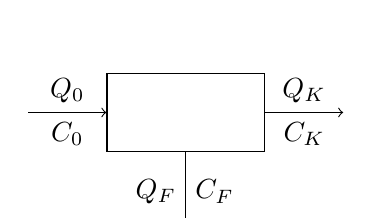
\begin{tikzpicture}
      % Box
      \node[draw, rectangle, minimum width=2cm, minimum height=1cm] (box) at (0, 0) {};
      % Arrows
      \draw[->] (-2, 0) -- (box.west) node[midway, above] {$Q_0$} node[midway, below] {$C_0$};
      \draw[->] (box.east) -- (2, 0) node[midway, above] {$Q_K$} node[midway, below] {$C_K$};
      \draw[->] (box.south) -- (0, -1.5) node[midway, left] {$Q_F$} node[midway, right] {$C_F$};
    \end{tikzpicture}
    \caption{Schematics for solids and fluid balance.}
    \label{fig:balance}
\end{figure}
where:\\
$0$ $\Rightarrow$ inflow (influent),\\
$K$ $\Rightarrow$ cake,\\
$F$ $\Rightarrow$ outflow (filtrate/centrate).\\
\textbf{Solids recovery:} how much of the incoming solids are captured in the cake, how little we are releasing to outflow.
\begin{equation}
    Q_0 = Q_F + Q_K
    \label{eq:liqbalance}
\end{equation}
\begin{equation}
    Q_0C_0 = Q_FC_F + Q_KC_K
    \label{eq:solidsbalance}
\end{equation}
Substituting Equation \ref{eq:liqbalance} into Equation \ref{eq:solidsbalance}:\\
$Q_0C_0 = Q_FC_F + Q_KC_K$\\
$Q_0C_0 = C_F(Q_0-Q_K) + Q_KC_K$\\
$Q_0C_0 = C_FQ_0-C_FQ_K+ Q_KC_K$\\
$Q_0 (C_0-C_F) = Q_K (C_K-C_F) $\\
Leaving $Q_K$ alone:
\begin{equation}
    Q_K=\frac{Q_0(C_0-C_F)}{(C_K-C_F)}
    \label{eq:balance}
\end{equation}
\% Recovery:
\[
\%R =\frac{\text{mass of dry solids as cake}}{\text{mass of dry feed solids}}*100
\]
\begin{equation}
    \%R =\frac{C_KQ_K}{C_0Q_0}*100
    \label{eq:recovery}
\end{equation}
Substituting Equation \ref{eq:balance} into Equation \ref{eq:recovery}:
\[
\%R =\frac{C_K(C_0-C_F)}{C_0(C_K-C_F)}*100
\]
where:\\
$Q_0$ = feed flow rate,\\
$C_0$ = feed solids concentration,\\
$Q_K$ = filter cake flow,\\
$C_K$ = filter cake solids concentration,\\
$Q_F$ = the filtrate flow,\\
$C_F$ = the solids concentration in the filtrate.
\begin{enumerate}
    \item Non-mechanical Dewatering
    \begin{enumerate}
        \item Drying beds\\
        Depth 15--30 cm, several weeks to months to dry. Sand and gravel structure.\\
        \textbf{Sludge collection:}\\
        manual $\Rightarrow$ better, more careful, but not aesthetically acceptable\\
        forklifts $\Rightarrow$ we lose sand\\
        Mechanisms:
        Water drains through sand until sand is clogged, there is a drainage system underneath. 25\% (if not conditioned), 75\% (with good conditioning) removal of water can be achieved.\\
        Evaporation dewatering does not much depend on sludge, it depends on climate and surface characteristics of sludge.\\
        \textbf{Disadvantages:} climate dependent, high land requirement.\\
        \textbf{Advantages:} small plants are good, low electricity, low requirement for operator attention\\
        \textbf{Design}\\
        Based on: solids loading rates kg/m$^2$/y\\
        Best way to design: pilot studies.\\
        Covered area requires less area due to less precipitation factor.
        \item Lagoons\\
        No under-drain system, very large volumes are required, depth around 1 m, an odor intensive process. Again precipitation should be accounted.
    \end{enumerate}
    \item Mechanical Dewatering
    \begin{enumerate}
        \item Pressure filters\\
        ``Filter press", not a right name, because not pressing. It is coming from ``pressure".\\
        Pressurized so that water is removed, cake is removed from the surface.\\
        \textbf{Disadvantages:} It is a cyclic oepration, very disadvantageous in large treatment systems, generally effective in smaller plants. Cleaning aspect since not aesthetically acceptable.\\
        Filter presses nicely dewater 50:50 (Digested P:S) to a solids concentration of 35 to 47\%\\
        Performance based on:
        \begin{itemize}
            \item solids content,
            \item chemical conditioning dose,
            \item cake solids content,
            \item total cycle time,
            \item solids capture,
            \item the desired yield (kg/y/m$^2$)
        \end{itemize}
        \textbf{Design}\\
        Based on: \emph{cake solids concentration}, \emph{yield rate}, \emph{recovery fraction}.\\
        Cycle time $\uparrow$ solids concentration in the cake $\uparrow$, but means reduced rate of throughput.\\
        95\% recovery is aimed.\\
        Sizing the dewatering equipment depends on the suppliers.
        \item Belt filter presses\\
        Very much loved in turkey, low capital system, versatile, low-speed.\\
        In S zone, shear and direction changes, 20--25\% achieved.
        \item Centrifuges\\
        High force 500--3000 G force so that solids are removed from the water, then sludge is scraped from the walls of the solid-bowl centrifuge (the type of machine used in wastewater treatment).\\
        Process variables: \emph{feed flow rate}, \emph{rotational speed}, \emph{different speed of the conveyor}, \emph{chemical use}, \emph{pond depth}, \emph{physicochemical properties}.\\
        Operation: solid bowl bullet shaped casing, which is outside scroll and a screw conveyor that is placed in the middle of the centrifuge.\\
        \textbf{Objectives:} \emph{dry cake}, \emph{clear centrate}, \emph{reasonable throughput} (\emph{centrifuge yield}).\\
        Clarification of the liquid, successful movement of the cake is achieved.\\
        Machine variables:
        \begin{itemize}
            \item Bowl diameter
            \item Bowl length
            \item Bowl speed
            \item Bowl angle
            \item Residence time
            \item Pool depth
            \item Conveyor speed
            \item Feed point of sludge
        \end{itemize}
        Operational (Sludge related) variables:
        \begin{itemize}
            \item Sludge type
            \item Solids concentration
            \item Conditioning
        \end{itemize}
        This method gives the strongest flocs, not necessarily the larger flocs. Floc strength can be measured by \emph{visually} or \emph{floc strength} tests which is intentionally shearing the sludge to break the flocs.\\
        Performance: \textbf{at least} 66\% solid recovery with 30--35 \% cake solids obtained. Lower feed solids are more efficient.\\
        Design: Depends on manufacturers and allowable loading.
    \end{enumerate}
\end{enumerate}

\begin{table}
\centering
\label{tab:dewatering_processes}
\caption{Comparison of different processes for dewatering.}
\begin{tabular}{p{4cm}p{5cm}p{5cm}}
\toprule
\textbf{Process} & \textbf{Advantages} & \textbf{Disadvantages} \\
\midrule
Centrifuge & relative less space, \newline clean appearance and good odor & relatively high costs, \newline direct energy usage \\
Belt filter press & easy to operate, \newline relatively low costs & very sensitive to feed sludge,\newline sensitive to the polymer \\
Pressure filter press & high cake solids concentration,\newline good with hardly dw. sludges & batch operation,\newline high capital and labor costs \\
Drying beds and lagoons & low capital costs,\newline low energy consumption & large area and stabilized sludge, \newline climate effect \\
\bottomrule
\end{tabular}
\end{table}
\date{\begin{flushright}May 26, 2023\end{flushright}}
\section{Chemical Sludges} \label{section:chemicalsludges}
Originating:
\begin{enumerate}
    \item Water $\Rightarrow$ different type of sludge (mostly alum)
    \item Wastewater (domestic) $\Rightarrow$ may be due to seasonal changes and small plants, BOD and SS removal can be achieved, hard to remove P with only this method in those plants, deep ocean disposal for sludge via chemically enhanced primary treatment (CEPT) can be applied.
    \item Wastewater (industrial) $\Rightarrow$ may be completely toxic.
\end{enumerate}
Chemical sludge properties:
\begin{itemize}
    \item high water quantity,
    \item hard to dewater,
    \item not reactive (except P removal sludge), which is the best part about them.
\end{itemize}
\textbf{Water Treatment (Alum) Sludge}
\begin{itemize}
    \item 98\% moisture
    \item BOD $\approx$ 50 mg/L
    \item COD $\approx$ 500 - 1500 mg/L
    \item pH $\approx$ 6
\end{itemize}
They are mostly treated as industrial sludges, landfilling.\\
\textbf{Properties:}
\begin{itemize}
    \item \textbf{Thickeners} $\Rightarrow$ may be used,
    \item \textbf{Rheologically} $\Rightarrow$ Newtonian fluids,
    \item \textbf{Dewatering} $\Rightarrow$ high SRF (hard to dewater),
    \item \textbf{Conditioning} $\Rightarrow$ chemical conditioning is effective, esp. if climate permits, such as freezing/thawing.
\end{itemize}
SRF $\downarrow$ as solid concentration $\uparrow$ in water sludges.\\
Dewatering applications:
\begin{itemize}
    \item Centrifuges
    \item Pressure filters
\end{itemize}
\textbf{Alum's Domestic Wastewater Applications:}\\
\ce{Al^3+ + PO_4^3- \rightleftarrows AlPO4} $\downarrow$ insoluble ppt. (excellent removal mechanism)\\
Sludge production formulas:\\
\ce{Al^3+ + PO_4^3- \rightleftarrows AlPO4} $\downarrow$ ppt.\\
\ce{Al^3+ + 3OH- \rightleftarrows Al(OH)3} $\downarrow$ ppt.\\
Total sludge produced $\sum (1 + 2)$
Reducing the pH (acidification) would result in \ce{Al^3+} recovery:\\
\ce{Al(OH)3 + 3H+ \rightarrow Al^3+ + H2O}\\
\textbf{Iron Sludge}\\
\ce{Fe^2+}: Ferrous in \ce{FeSO4} form, \ce{Fe^3+}: Ferric in \ce{FeCl3} form (better compared to ferrous).\\
\textbf{Properties:}
\begin{itemize}
    \item soft, fluffy
    \item 10--12 \% achievable solid concentration
    \item still behaves as fluid when concentrated
\end{itemize}
\ce{Fe^3+ + PO_4^3- \rightleftarrows FePO4} $\downarrow$\\
\ce{Fe^3+ + 3OH- \rightleftarrows Fe(OH)3} $\downarrow$\\
Total sludge produced $\sum (1 + 2)$\\
\textbf{Lime Sludge}\\
\ce{CaO}: Quicklime, \ce{Ca(OH)2}: Slaked/hydrated lime.\\
High pH generated ($\approx$ 11.5) $\rightarrow$ carbonates, phosphates, etc. will precipitate out.\\
Phosphorus removal achieved with \ce{Ca5(OH)(PO4)3} (calcium hydroxylapatite), flocs are small; therefore, hard to dewater.\\
\ce{CaO + H2O \rightleftarrows Ca(OH)2} (slacking reaction: sudden temperature increase, high pH, which is very effective sludge stabilization)\\
Nice soil conditioning for acidic soils (by achieving higher water holding capacity and permeability).\\
Disposal options for \textbf{Industrial (Toxic) Sludge}:
\begin{enumerate}
    \item \textbf{Deep well injection:} Way deep, two impervious/confined strata, downside: no way to reach the waste, it may come back to surface.
     \item \textbf{Landfill:} A dedicated landfill is a must.
     \item \textbf{Stabilization (Fixation) / Solidification:} Stabilization $\Rightarrow$ reduces toxicity; Solidification $\Rightarrow$ reduces mobility (ex. pozzolan + lime).
\end{enumerate}
\section{Sludge Drying and Combustion}
Beneficial use, also can be considered as final destination.\\
Thickening and dewatering do a potential job to help sludge drying, but 35\% is not enough. Thermal energy is required.\\
\textbf{Sludge Drying:} processing solid product with high organic content.\\
\textbf{Sludge Combustion:} converting the volatile solids into \ce{CO2} and \ce{H2O}.
\subsection{Drying}
\begin{figure}[htbp]
    \centering
    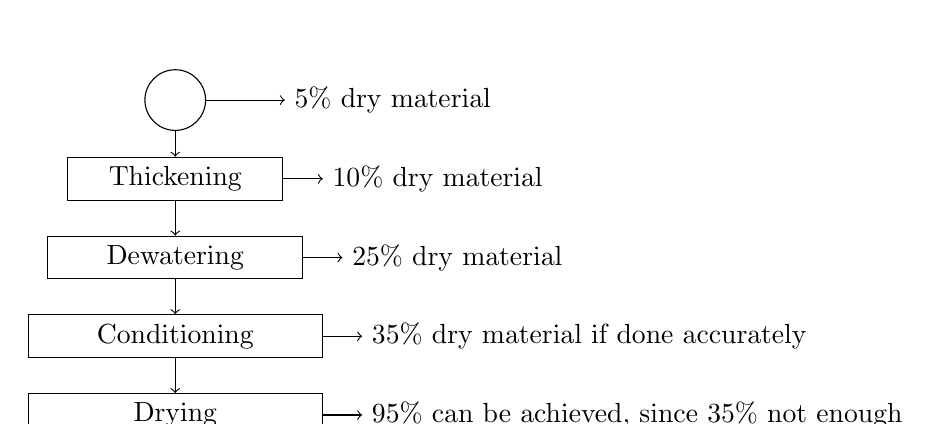
\begin{tikzpicture}[node distance=1cm, auto]
    % Circle: 
    \node[circle, draw, text width=0.5cm, align=center] (empty) {};
    \node[right=of empty] (emptyLabel) {5\% dry material};
    % Rectangle: Thickening
    \node[rectangle, draw, text width=2.5cm, align=center, below of=empty] (thickening) {Thickening};
    \node[right= 0.5 cm of thickening] (thickeningLabel) {10\% dry material};
    % Rectangle: Dewatering
    \node[rectangle, draw, text width=3cm, align=center, below of=thickening] (dewatering) {Dewatering};
    \node[right= 0.5 cm of dewatering] (dewateringLabel) {25\% dry material};
    % Rectangle: Conditioning
    \node[rectangle, draw, text width=3.5cm, align=center, below of=dewatering] (conditioning) {Conditioning};
    \node[right= 0.5 cm of conditioning] (conditioningLabel) {35\% dry material if done accurately};
    % Rectangle: Drying
    \node[rectangle, draw, text width=3.5cm, align=center, below of=conditioning] (drying) {Drying};
    \node[right= 0.5 cm of drying] (dryingLabel) {95\% can be achieved, since 35\% not enough};
    % Arrows
    \draw[->] (empty) -- (thickening);
    \draw[->] (thickening) -- (dewatering);
    \draw[->] (dewatering) -- (conditioning);
    \draw[->] (conditioning) -- (drying);
    \draw[->] (empty) -- (emptyLabel);
    \draw[->] (thickening) -- (thickeningLabel);
    \draw[->] (dewatering) -- (dewateringLabel);
    \draw[->] (conditioning) -- (conditioningLabel);
    \draw[->] (drying) -- (dryingLabel);
    \end{tikzpicture}
    \caption{Sludge treatment stages and their respective achieved dry material percentages.}
    \label{fig:sludge_stages}
\end{figure}


Sludge Drying Stages:
\begin{enumerate}
    \item Warming up: Increasingly drying, short stage.
    \item Constant Rate: The evaporation and the inside movement are in the same rate.
    \item Falling rate: Not a fixed slope, drying rate decreases.
\end{enumerate}
Moisture content affects the drying rate!\\
Sludge Drying Stages Based on Water Types:
\begin{enumerate}
    \item Free water: Constant rate
    \item Interstitial water: First falling rate, linearly
    \item Surface water: Second falling rate, logarithmic
\end{enumerate}
Thermal dryer types:
\begin{itemize}
    \item convective or direct dryers,
    \item conductive or indirect dryers
    \item mixed systems
\end{itemize}
\textbf{Direct sludge dryers:}\\
Direct contact (\textsl{convective}) of sludge with the heating agent such as hot gases from the combustion of an external fuel, alternatively dried sludge can be contacted with the dewatered cake in the drier to evaporate the remaining water.\\
\textbf{Advantages:} Simpler in design, effective systems.\\
\textbf{Disadvantages:} Higher temperatures, often have problems associated with dust and odors.\\
Very intensive systems!\\
\textbf{Indirect sludge dryers:}\\
Predominantly \textsl{conductive} systems.\\
\textbf{Advantages:} Reduced odor and dust, reduced air pollution problems.\\
\textbf{Disadvantages:} a little less efficient due to longer drying times.\\
Investment and operation are costly in both cases!\\
\textbf{Solar drying:}\\
Almost comes to 60--80 \% solid content, 90\% cannot be achieved (Mallorca example). A greenhouse type of structure with air movement, mixing etc. Large area requirement, takes time, ambient moisture level and in the atmosphere is critical. They are not really cheap options due to land cost. The system is so mechanic as well.
\subsection{Combustion/Incineration}
\textbf{Incineration:} Full oxidation (combustion of wastes), \textbf{combustion} might be partial. Drying is a crucial step to provide efficiency.\\
Sludge has organic content but also high water content.\\
It is an expensive process (esp. in drying part).\\
The heat value depends on the elemental composition of the sludge, this determines whether the auxiliary fuel will be needed or not.\\
The stabilization reduces the calorific value dramatically.\\
\textbf{Heat value of sludge:}
\begin{itemize}
    \item Elemental composition can be used in \textsl{Dulong's formula}.
    \item Calorimeter measurements can be applied for an experimental approach.
    \item Empirical formulas can also be used from the literature.
\end{itemize}
H.C.V. or H.H.V. calculations:
\[
\text{kJ/kg} = 33800 C + 144000 (H - O/8) + 9270 S
\]
\[
\text{BTU/lb} = 14600 C + 62000 (H - O/8) + 4050 S
\]
\[
\text{kcal/kg} = 8080 C + 34500 (H - O/8) + 2240 S
\]
where:\\
C, H, O, S are the weight fractions of corresponding elements.\\
Conversions:
\[
\text{BTU/lb} = \frac{\text{kJ/kg}}{2.326}
\]
\[
\text{kcal/kg} = \frac{\text{kJ/kg}}{4.184}
\]
\[
\text{kcal/kg} = \frac{\text{BTU/lb}}{1.799}
\]
Some empirical formulas can be used to determine the heat value as well:
\[
Q_H = A\left[\frac{100C_V}{100-D}\right] - B\left[\frac{100-D}{100}\right]
\]
or such as,
\[
\text{BTU/lb} = 122C_V - 660
\]
where:\\
$Q_H$ = heat value (BTU/lb),\\
$C_V$ = volatile solids (\%),\\
$D$ = dosage of inorganic chemicals used in dewatering as \% weight of sludge,\\
$A$ = empirical constant (107 for Activated Sludge, 131 for Raw Primary Sludge),\\
$B$ = empirical constant (5 for Activated Sludge, 10 for Raw Primary Sludge).\\
Even though the calorific value of sludge ($\approx$ 5500 kcal/kg) compared to coal and oil ($\approx$ 7800 kcal/kg and $\approx$ 10600 kcal/kg) looks good, the water content ($\approx$ 80\%) and non-volatile portion ($\approx$ 30\%) of the sludge should be accounted.
\[
\text{Real Heat Value} = \text{Heat Value} * f_S * f_V
\]
where:\\
$f_S$ = solid fraction ($\approx$ 0.2--0.25),\\
$f_V$ = volatile fraction ($\approx$ 0.7).\\
To increase the heat value of sludge: \emph{dewatering aids} and \emph{co-combustion with other wastes}.
Combustion systems:
\begin{enumerate}
    \item Multiple Hearth Incinerator
    \item Fluidized Bed Incinerator
    \item Rotary Kiln Incinerator
\end{enumerate}
\textbf{Multiple Hearth Incinerator}\\
Horizontal shelves (hearths), dropping sludge, upper for vaporization, middle for burning, and lower for the cooling off.\\
Air goes the other way (countercurrent).\\
\textbf{Fluidized Bed Incinerator}\\
Fluidizing medium (preheated sand), completely mixed with a medium. Suspension, very homogeneous, very efficient!\\
Excess air (20\%) is needed, which means air pollution control.\\
\textbf{Rotary Kiln Incinerator}\\
Very high temperatures, 2 stage, with inclination the sludge moves while rotating.\\
Two important factor:
\begin{enumerate}
    \item Calorific value
    \item Moisture content
\end{enumerate}
If the following are provided adequately, a succesful incineration happens:
\begin{enumerate}
    \item Time,
    \item Temperature,
    \item Turbulence (3Ts of combustion),
    \item Oxygen,
    \item Constant and adequate feed.
\end{enumerate}
Excess air is always needed ($\approx$ 50--100 \%).
\subsection{Air pollution issue}
One problem: air pollution control, due to ash and odor problems.\\
\textbf{Air pollution control units} are a must.
Two major constituents:
\begin{enumerate}
    \item Particulates and flue gas stream
    \item Acid gases
\end{enumerate}
Particulate removal:
\begin{enumerate}
    \item Gravity separation
    \item Interference
    \item Centrifugal separation
    \item Filtration
    \item Electrostatic separation
    \item Wetting a particle with water and then ``scrubbed" (both wet or dry systems except this one)
\end{enumerate}
Acid gas removal (\ce{HCl} and \ce{SO2} are neutralized and salty water is handled):
\begin{enumerate}
    \item Dry lime injection
    \item Dry scrubber (those are dry)
    \item Absorption/reaction
    \item Wetting contactors (wet options)
\end{enumerate}
\textbf{Alternative Thermal Treatment Technologies}\\
\textit{Gasification}\\
Kinda like \textit{pyrolysis} (no oxygen introduction), some oxygen input (limited): syngas (is a mixture of hydrogen and carbon monoxide, in various ratios; the gas often contains some carbon dioxide and methane), char or slag, oils and reaction water is produced.\\
Wastewater sludge can act as a raw material or an energy source in cement kilns (moisture content is a problem).
\date{\begin{flushright}June 2, 2023\end{flushright}}
\section{Beneficial Use / Ultimate Disposal of Sludge}
\subsection{Beneficial Use and Disposal Methods}
Beneficial use increased overall, disposal is reduced throughout the years.\\
Land application takes a huge portion of the beneficial use. Disposal can include incineration.
Pathways:
\begin{enumerate}
    \item Air $\Rightarrow$ combustion and incineration.
    \item Land (two application): landfilling $\Rightarrow$ disposal; land application $\Rightarrow$ beneficial.
    \item Water $\Rightarrow$ sea/ocean disposal.
\end{enumerate}
\textbf{Ocean Disposal}\\
Very recently until in England, 2000s still done. A bad example. The countries which are closed to ocean applied this. Removal mechanisms during sea disposal: waves (\emph{dilution}), \emph{decay} and \emph{dispersion}.\\
\textbf{Typical problems:}
\begin{itemize}
    \item \emph{Stratification} problem: mixing not happening\\
    Large volumes deplete oxygen, will settle to the bottom, bottoms will turn \textbf{anaerobic}. In NY, 50 km$^2$ is dead sea.
    \item Metal was accumulated in fish \& shellfish.
\end{itemize}
Turkey did it before EU (1998), in \textbf{1988} with US by \textbf{Water Pollution Control Regulations}.\\
England is a great example due to the dramatic shift to land application.\\
\textbf{Land Applications} $\Rightarrow$ fertilizer and soil conditioner.\\
\textbf{Soil conditioner:} water holding capacity, porosity, permeability, pH.\\
Two ways of applying:
\begin{enumerate}
    \item Solidifying sludge $\rightarrow$ Trucks $\rightarrow$ Lay over the land
    \item Liquid sludge $\rightarrow$ nozzle trucks
\end{enumerate}
Where:
\begin{enumerate}
    \item Agricultural lands $\Rightarrow$ food, feed and fiber crops
    \item Pasture and rangeland
    \item Public contact sites $\Rightarrow$ parks and golf courses
    \item Non-agricultural areas such as forests
    \item Disturbed lands $\Rightarrow$ mine spoils, construction sites, gravel pits
    \item Superfund sites (locations polluted with hazardous materials) for reclamation
    \item Dedicated land disposal sites
    \item Home lawns and gardens
\end{enumerate}
How much? Not a question for us.\\
It is good soil additive but not a good soil to grow plants (esp. ammonia is toxic to plants at high concentrations).\\
Stages:
\begin{enumerate}
    \item Preliminary Planning Process $\Rightarrow$ Public participation, land area requirement, sludge transport.
    \item Site Screening $\Rightarrow$ Land availability, aesthetics, site acquisition, physical factors evaluation, contact with the owner.
    \item Site Evaluation (more detailed): Topographical limitations, soil characteristics, delineation of flood plaints, site hydrology, land application rates, land application practices, cost estimation, final site selection
\end{enumerate}
Things to be considered:
\begin{enumerate}
    \item Agronomic rates (nitrogen, phosphorus and potassium needs)!
    \item Potential harms and dangers! (such as pathogens and many organic substances, but these can be solved by sunlight, soil microorganisms and desiccation)
\end{enumerate}
Potential problems:
\begin{enumerate}
    \item Odor - major problem
    \item Transmittal of toxins (metals, hazardous organics, pathogens) into water supplies
    \item Transfer of pathogens - translocation of chemicals to crops which are consumed by animals.
    \item Detrimental effects on crops - such as high concentration of ammonia stop seed germination and causing toxicity.
\end{enumerate}
\subsection{Concerns}
\textbf{Heavy metals}\\
In purely domestic, it is in low amounts, but even controlled municipal (includes commercial and industrial wastewater) the amounts increases dramatically. Pre-treatment reduces the heavy metals in the sludge.\\
For the land application, the tolerance of the plants varies. Since heavy metals are micro-nutrients, they might help the growth. But these accumulate in the plants.\\
\textbf{Uptake depends on:} \emph{plant type}, the \emph{heavy metal type}, the \emph{application rate}.\\
\textbf{Total body burden concept} (decided by EPA, sourced from food, atmosphere etc.):
\ce{Pb} $>$ \ce{Cd} (\ce{Pb} can be exposed more), \ce{Cd} is highly and more toxic, \ce{Cd} poisoning $\Rightarrow$ ouch-ouch disease.\\
\textbf{Pathogenic microorganisms}\\
No guarantee 100\% removal, so there is a risk.\\
Dilution effect brings to the regulatory limits.\\
Pathways are critically important. Direct ingestion, aerosol transport etc.\\
\textbf{Trace organics} (Newer concerns, check page \pageref{CurrentIssues} for the full list of \textit{Current Issues})\\
Really low concentrations, such as PCBs, pesticides and oil/grease, etc.\\
They are hard to degrade, persistent contaminants. Bio-magnification (accumulation in the fat tissues) is a serious issue.\\
These are emerging contaminants, their effects started to show up.\\
PPCP: Pharmaceuticals and personal care products.\\
What can be done?\\
\textbf{Best effective way:} Source control with restriction.\\
\textbf{Landfilling}\\
As a disposal method, not sustainable.\\
\textbf{Disadvantages:} disposing \emph{a valuable resource}, filling up \emph{landfill sites rapidly}, \emph{generating gas} which is usually not controlled.
\date{\begin{flushright}June 9, 2023\end{flushright}}
\section{Regulations of Sludge}
\subsection{Turkish Regulations}
\begin{enumerate}
    \item \textbf{Su Kirliliği Kontrol Yönetmeliği (Water Pollution Control Regulations):} First regulation that forbids sludge disposal to water bodies.\\
    First September 4, 1988, then revised.
    \item \textbf{Atıksu Arıtma Tesisleri Teknik Usuller Tebliği (WPCR -- Technical Aspects Bulletin):} Very technical document! All the technicality for the sludge treatment are given in the document.
    \item \textbf{Atıkların Düzenli Depolanmasına Dair Yönetmelik\\(Regulation on the Landfilling of Wastes)}\\
    Three types of landfills:
    \begin{enumerate}
        \item Hazardous waste
        \item Municipal waste
        \item Inert waste
    \end{enumerate}
    Those are determined by the analysis.\\
    Different types has different limiting values.\\
    Treatment might be required before the disposal.\\
    Dissolved Organic Carbon (DOC) is a critical parameter since it makes the waste reactive. DOC $\Rightarrow$ The requirement goes further because it is not easy to eliminate organic activity.\\
    The organic content reduction is aimed for 35\% until 2025 $\Rightarrow$ can be achieved by more digestion.
    \item \textbf{Atıkların Yakılmasına Dair Yönetmelik (Regulation on the Combustion of Wastes):}\\
    Mono $\Rightarrow$ no need auxiliary fuel, if more than 40\%.\\
    If not, auxiliary fuel is needed, which is called co-incineration.
    \item \textbf{Evsel ve Kentsel Arıtma Çamurlarının Toprakta Kullanılmasına Dair Yönetmelik (Regulation on the Use of Municipal and Urban Sludges on Land):} Great regulations, every line is about sludge.\\
    But no land application is implied in Turkey.\\
    A very strict based on safety and hygiene! Every characteristics of sludge is listed and the conventional values are really strict! Additionally, some extra organic compounds (different than EU) are restricted as well. \emph{Heavy metals}, \emph{toxic compounds}, \emph{emerging contaminants} and \emph{microbial organisms} are included. Even after application, every \textbf{12 months period}, analyzing the soil is mandatory.
\end{enumerate}
\subsection{US Regulations}\label{regulation:us}
Regulated under \textbf{Federal Regulation in 40 CFR Part 503 Standards for the Use or Disposal of Biosolids}. There are previous versions. The 503 establishes for standards for the final use of disposal of sewage sludge, whether agricultural or non-agricultural.\\
\textbf{Vector attraction} (which are disease carriers) is mentioned in this one and it is a huge part of the sludge storage. \emph{Monitoring}, \emph{record-keeping} and \emph{reporting} are done in regular bases.
\begin{itemize}
    \item Subpart A -- General Provisions
    \item Subpart B -- Land Applications $\Rightarrow$ nice comparison!
    \item Subpart C -- Surface Disposal
    \item Subpart D -- Pathogen and Vector Attraction Reduction $\Rightarrow$ important!
    \item Subpart E -- Incineration
\end{itemize}
Very specific ceiling concentrations such as heavy metals, vector reduction and pathogens. Since it is trusted and safe, it is sold!\\
Besides one time application values, there is cumulative loading rate for the site.
Not applied on a site if:
\begin{enumerate}
    \item Adversely affect a threatened or endangered species $\Rightarrow$ same as Turkish.
    \item The field is flooded, frozen or snow-covered.
    \item the application site is within 10 meters.
\end{enumerate}
\textbf{A label} will be affixed to the bag or container. All the information is given on that label.\\
\textbf{Operational Standards:} Pathogen \& Vector Attraction reductions are the base.
Pathogens:\\
Class A: very safe, best quality, kids can be around!\\
Class B: at least 1 month site restriction.\\
Vector Attraction:\\
Done for the storage period, mostly!\\
Should be met when applied or in: agricultural land, forest, public contact sites; lawns or home gardens; a bag or container.\\
For the pathogen count: MPN / g TS (dry). Class A has low values but not zero!\\
Best way to vector attraction reduction: Digestion, since it is desired to reduce the organic content in the sludge!\\
The mass of VS should be decreased by 38\%. Cannot be achieved aerobically, and if not in anaerobically, extra days and high temperature should be supplied. The specific oxygen update rate (SOUR) for sewage sludge must be \textbf{1.5 mg \ce{O2}/h/g TS}.
\printbibliography[heading=bibintoc]
\label{LastPage}
\end{document}